%-------这是COMAP公司发布的2023年美赛官方LaTeX模板
%-------官方仅提供了summary页面的样式,在此基础上,我们构建一个完整的Template!
%-------下载网站:https://www.comap.com/contests/mcm-icm
%-------E-mail:hnuzyx@outlook.com
%%%%%%%%%%%%%%%%%%%%%%%%%%%%%%%%%%%%%%%%
%% MCM/ICM LaTeX Template %%
%% 2023 MCM/ICM           %%
%%%%%%%%%%%%%%%%%%%%%%%%%%%%%%%%%%%%%%%%
\documentclass[12pt]{article}
\usepackage{geometry}
\geometry{left=1in,right=0.75in,top=1in,bottom=1in}

%%%%%%%%%%%%%%%%%%%%%%%%%%%%%%%%%%%%%%%%
% Replace ABCDEF in the next line with your chosen problem
% and replace 1111111 with your Team Control Number
\newcommand{\Problem}{C}
\newcommand{\Team}{2416613}
%%%%%%%%%%%%%%%%%%%%%%%%%%%%%%%%%%%%%%%%
\usepackage{algorithm}
\usepackage{algpseudocode}
\usepackage{newtxtext}
\usepackage{hyperref}
\usepackage{amsmath,amssymb,amsthm}
\usepackage{lipsum}
\usepackage{booktabs}
\usepackage{float}

\usepackage{listings}
\usepackage{fancyhdr}
\usepackage{appendix}
\usepackage{indentfirst} % 首行缩进
\usepackage{enumitem}  % 无序列表样式
\usepackage{subfigure}  % 子图
\usepackage[T1]{fontenc}  % 为了能识别双直引号
\usepackage{algorithmicx}  % 伪代码
\usepackage{algpseudocode}
\renewcommand{\algorithmicrequire}{ \textbf{Input:}}     %Use Input in the format of Algorithm
\renewcommand{\algorithmicensure}{ \textbf{Output:}}    %UseOutput in the format of Algorithm
\usepackage[pdftex]{graphicx}
\usepackage{xcolor}
\usepackage{fancyhdr}
\usepackage{url}
\lhead{Team \Team}
\rhead{}
\cfoot{}

\hypersetup{
	colorlinks=true,
	linkcolor=black
}

% 设置listings宏包的参数
\lstset{
  language=Python, % 设置语言为C语言,根据需要可以设置为Python、Java等
  basicstyle=\sffamily, % 设置代码字体
  keywordstyle=\color{pink}, % 设置关键字颜色
  commentstyle=\color{green}, % 设置注释颜色
  % stringstyle=\color{red}, % 设置字符串颜色
  showstringspaces=false, % 不显示字符串中的空格
  breaklines=true, % 自动折行
  frame=single, % 添加边框
}

\lstset{
    numbers=left, 
    numberstyle= \tiny, 
    breaklines=true, % 自动折行
    keywordstyle= \color{ blue!70},
    commentstyle= \color{red!50!green!50!blue!50}, 
    frame=shadowbox, % 阴影效果
    rulesepcolor= \color{ red!20!green!20!blue!20} ,
    escapeinside=``, % 英文分号中可写入中文
    xleftmargin=2em,xrightmargin=2em, aboveskip=1em,
    framexleftmargin=2em
} 

\fancypagestyle{nopagenum}{
  \fancyhf{} % 清空当前设置
  \fancyhead[L]{Team 2416613}
  \fancyhead[R]{\thepage}
  % \fancyfoot[L]{} % 左脚注
  % \fancyfoot[C]{} % 中脚注
  % \fancyfoot[R]{} % 右脚注
  \renewcommand{\headrulewidth}{0.4pt} % 页眉线宽,设为0可以去掉页眉线
  \renewcommand{\footrulewidth}{0.4pt} % 页脚线宽,设为0可以去掉页脚线
}

\newtheorem{theorem}{Theorem}
\newtheorem{corollary}[theorem]{Corollary}
\newtheorem{lemma}[theorem]{Lemma}
\newtheorem{definition}{Definition}

%%%%%%%%%%%%%%%%%%%%%%%%%%%%%%%%
\begin{document}
\graphicspath{{.}}  % Place your graphic files in the same directory as your main document
\DeclareGraphicsExtensions{.pdf, .jpg, .tif, .png}
\thispagestyle{empty}
\vspace*{-16ex}
\centerline{\begin{tabular}{*3{c}}
	\parbox[t]{0.3\linewidth}{\begin{center}\textbf{Problem Chosen}\\ \Large \textcolor{black}{\Problem}\end{center}}
	& \parbox[t]{0.3\linewidth}{\begin{center}\textbf{2024\\ MCM/ICM\\ Summary Sheet}\end{center}}
	& \parbox[t]{0.3\linewidth}{\begin{center}\textbf{Team Control Number}\\ \Large \textcolor{black}{\Team}\end{center}}	\\
	\hline
\end{tabular}}
%%%%%%%%%%% Begin Summary %%%%%%%%%%%
% Enter your summary here replacing the (red) text
% Replace the text from here ...
% \begin{center}
%标题
\begin{center}
	\Huge {MM-LSTM: A Momentum LSTM Model for Tennis Match Prediction and Analysis}
	\vspace{0.4cm}
	
	\normalsize\textbf{Summary}
\end{center}
\vspace{0.2cm}

%下述段落为官方注意事项,写作时注意删除!
% \textcolor{red}{%
% Use this template to begin typing the first page (summary page) of your electronic report. This \newline
% template uses a 12-point Times New Roman font. Submit your paper as an Adobe PDF \newline
% electronic file (e.g. 1111111.pdf), typed in English, with a readable font of at least 12-point type.	\\[2ex]
% Do not include the name of your school, advisor, or team members on this or any page.	\\[2ex]
% Papers must be within the 25 page limit.	\\[2ex]
% Be sure to change the control number and problem choice above.	\\
% You may delete these instructions as you begin to type your report here. 	\\[2ex]
% \textbf{Follow us @COMAPMath on Twitter or COMAPCHINAOFFICIAL on Weibo for the \newline
% most up to date contest information.}
% }
% \end{center}
% to here


%生成随机段落,写作时删除这排语句即可!
% \lipsum[1-3]
Tennis is a widely acclaimed sport, and during matches, incredible swings often occur due to "momentum" which cannot be directly observed. To investigate the existence of this "momentum" and predict its trends, we utilize our \textbf{innovative MM-LSTM model} to model players' match states.

% For problem 1, we analyze the \textbf{Spearman correlation coefficients} among various parameters in tennis matches and dimensionally reduce the data based on these correlations. We employ \textbf{the MM-LSTM (Momentum--Long Short-Term Memory) model} to capture the \textbf{sequential variation} in the game, simulating the player's match state through its Cell state, Input Gate, Forget Gate, and Output Gate. This allow us to observe the current match situation, forget past situations, and account for hitting actions. The model's performance is validated on the test set, \textbf{achieving a loss value of 0.047 and an impressive accuracy of 94.52\%.}

For problem 1, we analyze the \textbf{Spearman correlation coefficients} among various parameters in tennis matches and dimensionally reduce the data based on these correlations.We employ \textbf{the Momentum-Long Short Term Memory (MM-LSTM) model} to model the \textbf{sequential variation} in the match. Its Cell state, Input Gate, Forget Gate, and Output Gate are used to simulate the player's match status, observations of the current match situation, forgetting past match situations, and the action of hitting the ball, respectively. Based on its output, we can judge the player's performance. The model's performance is validated on the test set, achieving a loss value of \textbf{0.047} and an impressive accuracy of \textbf{94.52\%}.


% For problem 2, we conduct \textbf{forward derivation}, \textbf{excluding momentum} and considering various factors' impact on predicting probabilities and establishing a \textbf{random probability model}. Using the MM-LSTM model as a starting point, we then \textbf{reverse-explain  the rationale} behind the random probability model. Testing both models on the same dataset reveals the MM-LSTM model's superior accuracy, \textbf{outperforming the random probability model by 26 percentage points with a remarkable accuracy of 94.23\%.}

For problem 2, we first conducted a \textbf{forward derivation}, \textbf{disregarding the momentum} and considering the impact of various factors on the predictive probability, thus establishing a \textbf{stochastic probability model}. Then, using the MM-LSTM model as a starting point, we \textbf{reverse-explain  the rationale} behind the stochastic probability model. We tested these two models on the same dataset. In the final results, the MM-LSTM model achieved a significantly higher prediction accuracy than the stochastic probability model, with an \textbf{improvement of 26 percentage points} at \textbf{94.23\%}. This clearly illustrates the importance of momentum.


% For problem 3, we delve beyond the surface of the MM-LSTM model, discovering a subtle relationship between\textbf{ the gradient of the function representing the relative score difference of athletes and their relative momentum} and use it as an indicator representing the progress of the game. Considering the connection between score changes and predicted probabilities, we bridge the gap with \textbf{probability transitions}. Conducting a \textbf{gradient importance analysis} on all input factors, we calculate the partial derivatives of inputs to outputs to assess each indicator's impact on momentum. Based on this analysis, we propose \textbf{5} effective recommendations.

For problem 3, we delve beyond the surface of the MM-LSTM model, discovering a subtle relationship between\textbf{ the gradient of the function} representing the relative score difference of athletes and their relative momentum and use it as an indicator representing the progress of the game. We considered the relationship between score changes and predicted probabilities, and established a bridge to represent momentum through \textbf{probability transition}. Taking more factors into account, we conducted a \textbf{gradient importance analysis} for all input factors. By calculating the partial derivatives of the input to the output, we determined the impact of various indices on momentum. Based on this, we proposed \textbf{5} effective recommendations.

For problem 4, we compare the MM-LSTM model's probability output \textbf{predictions} with the \textbf{actual} values of the mentioned tennis match,achieving an accuracy of \textbf{ 90.71\% }and \textbf{visualizing the fitting curve} between predicted and real values. Additionally, we expand the model to include factors from both \textbf{subjective and objective }perspectives, \textbf{such as environmental conditions and psychological traits}. Lastly, we collect 2024 WTT table tennis match data and evaluate the \textbf{generalizability} of our MM-LSTM model to \textbf{table tennis}, finding that the model's performance did not match that of tennis due to the smaller dataset and insufficient description of match states. Increasing the amount of data will bring more improvement in model performance.

Finally, we draft a memorandum summarizing our research findings, demonstrating the role of momentum in matches for coaches, and providing detailed advice for players on handling momentum.

%关键词
\vspace{0.4cm}
\noindent \textbf{Keywords: }Momentum \quad LSTM \quad  Gradient  
%%%%%%%%%%% End Summary %%%%%%%%%%%

%%%%%%%%%%%%%%%%%%%%%%%%%%%%%%
\clearpage
\pagestyle{fancy}
% Uncomment the next line to generate a Table of Contents
%\tableofcontents 
\newpage
\setcounter{page}{1}
\rhead{Page \thepage~of~25}
%%%%%%%%%%%%%%%%%%%%%%%%%%%%%%
%目录
\tableofcontents
\newpage

%正文部分
% \input{body/MCM-ICM_Summary}
\section{Introduction}
% \lipsum[1-8]
\subsection{Problem Background}

Tennis has always been a sporting event that is watched by the masses and in the men's final of the 2023 Wimbledon Tennis Championships, 20 year old Spanish star Carlos Alcaraz defeated 36 year old Novak Djokovic in a tightly contested match. At the start of the match, Djokovic showed overwhelming power that seemed to signal an easy victory. But the match took a surprisingly volatile turn during the course of the match. In the end it was Carlos Alcaraz, who was not favored at the start of the match, who emerged victorious.

\subsection{Problem Restatement}

\begin{figure}[h]
    \centering
    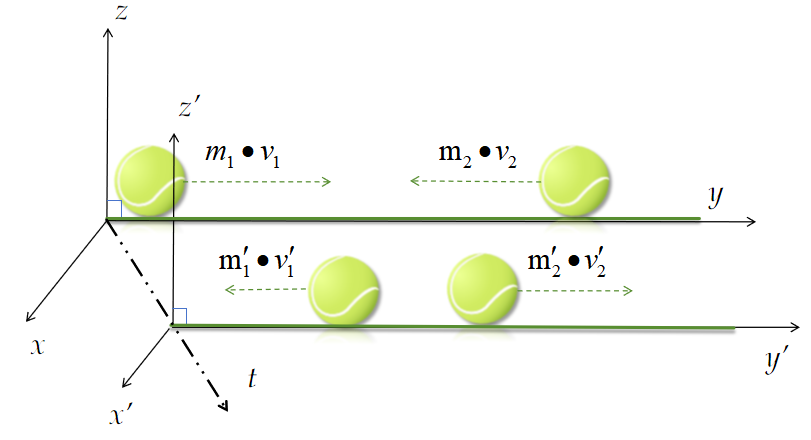
\includegraphics[width=0.7\textwidth]{figure/collision_of_tennis_balls(2).png}
     % \vspace{-0.3cm}
    \caption{The Momentum of Tennis}
    \label{fig:correlation_heatmap }
    % \vspace{-0.5cm}
\end{figure}
% 




Match swings are often linked to a player's momentum — the power or advantage gained. It's unclear how this momentum is generated or altered, prompting an examination of its role in matches and its predictive potential.

Given data from the 2023 Wimbledon Gentlemen's matches, including match ID, players' names, and elapsed time, we aim to use momentum observations to address the following problem:

\begin{itemize}[label=$\bullet$]
  \item Establish a model capable of analyzing player performance during a match, based on which the match process can be visualized and logically represented.
  \item Establish a traditional random probability model for comparison, assessing the role of momentum in the match.
  \item Analyze factors influencing turning points in a match from the following two perspectives:
    \begin{itemize}[label=\textbullet, itemsep=1ex]
       \item Develop a model for predicting match swings to analyze influencing factors.
       \item Provide players with recommendations to improve their chances of winning.
     \end{itemize}
 \item Evaluate the established predictive model for match swings based on the following two criteria:
    \begin{itemize}[label=\textbullet, itemsep=1ex]
       \item Analyze the accuracy of swing predictions, considering factors that may contribute to improving the model's accuracy when performance is subpar.
       \item Consider adding additional factors to enhance the model's generalizability.
    \end{itemize} 

\end{itemize}

\subsection{Our Work}
%%%%%%%%%%%%%%%%%%%%%%
%%% TODO
%%%%%%%%%%%%%%%%%%%%%%

\begin{figure}[h]
    \centering
    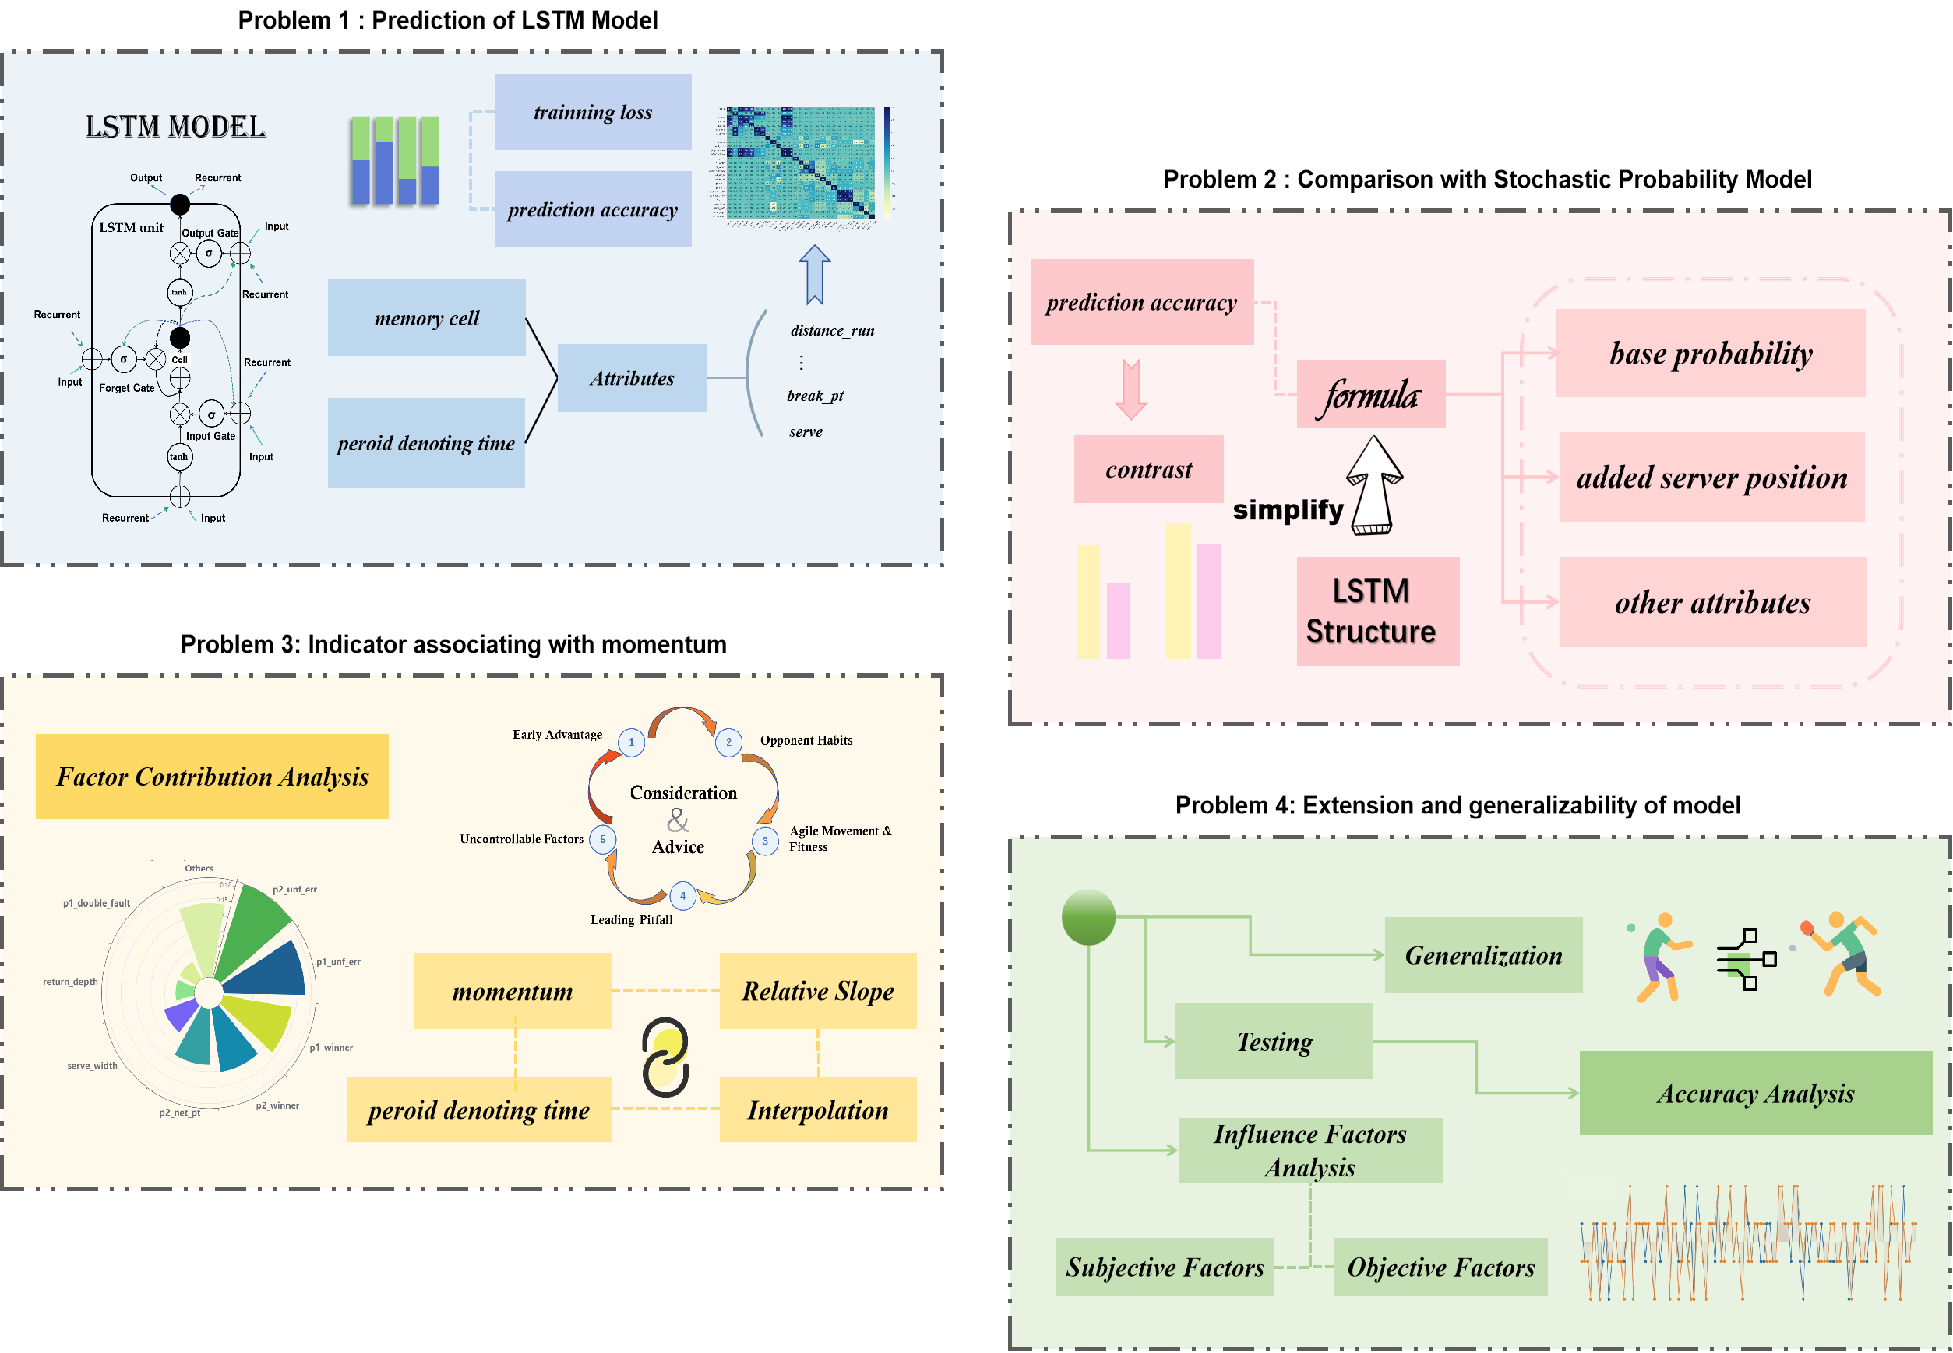
\includegraphics[width=1\textwidth]{figure/3.png}
     % \vspace{-0.3cm}
    \caption{Overall Architecture Diagram}
    % \vspace{-0.5cm}
\end{figure}

% 在问题一中,我们依据动量随时间的变化这个条件选取LSTM作为基础模型建模,重点观察动量的时间变化特点。首先我们对给定数据中字符串值的数据进行数字化,然后再归一化,去掉量纲。接下来我们分析了各种指标之间的相关性,选取其中独立性相对较强的部分,作为LSTM模型的输入,同时将数据集划分为训练集和测试集,经过大约六个小时的训练,得到准确率极高的模型输出。

In problem 1,\textbf{ we select LSTM as the foundational model based on the condition of momentum changing over time}, focusing on observing the temporal characteristics of momentum. Firstly, \textbf{we digitize the string values in the given data, followed by normalization to remove scale differences. }Subsequently, we analyze the correlations among various indicators, selecting those with relatively strong independence as inputs for the MM-LSTM model. Additionally, we divide the dataset into training and testing sets. After about 6 hours training, we obtain a highly accurate model output.

% 问题二要求我们以随机概率模型进行预测计算,与第一问的模型进行对比。我们首先对LSTM模型的原理进行剖析,整理得到其计算的核心公式,再通过对公式的抽象简化,得到可计算的简化的传统概率模型,同时降低了计算的复杂度。在这个模型中我们继续减少影响因素的个数,尽管计算得到的概率较低,但是相对于估计的真实的概率偏差不太大。同样这也说明了动量对于比赛得分的重要性。

In terms of problem 2, we conduct predictive calculations \textbf{using a random probability model and compare it with the model in problem 1}. We begin by analyzing the principles of the LSTM model,\textbf{ extracting its core formulas, and then abstracting and simplifying these formulas to obtain a computationally simplified traditional probability model}. This approach reduces computational complexity while maintaining calculability. In this model, we further reduce the number of influencing factors. Despite obtaining lower probabilities, the deviation from the estimated true probabilities is relatively small. This also underscores the significance of momentum in determining match scores.

% 经过我们对问题三题干的分析,相较于选择其他复杂因素的预测思路,我们剖析潜藏在历史胜负洪流中微不可查的动量变化。经过精密的数学推导,最终我们得到斜率相对差与动量之间的关系,发现了动量的变化原因和预报条件。同时我们也在训练中同步进行梯度重要性分析,得到影响准确性的主要因素。基于这些和对数据的分析计算,我们对运动员提出了基于“动量”的建议。我们对比赛开始以及过程中的动量波动分析,又对物理因素进行计算,最终总结提出五条有效建议。

After our analysis of the problem 3 prompt, in contrast to choosing prediction approaches involving other complex factors,\textbf{ we dissect the subtle momentum changes hidden within the historical win-loss dynamics}. Through precise mathematical derivations, we ultimately \textbf{establish the relationship between the relatively differential slope and momentum, uncovering the reasons for momentum changes and forecasting conditions.} Simultaneously, we conduct gradient importance analysis during training to identify the primary factors influencing accuracy. Based on these analyses and computations, we propose recommendations for athletes based on momentum. We compare momentum swings during the start and throughout the match, perform calculations related to physical factors, and ultimately summarize and \textbf{present five effective suggestions}.

% 在解决问题4的时候,我们首先使用LSTM模型预测的结果来绘制动量波动图像,并且计算出超过90%的准确性,证明了模型的优秀。同时我们在原本的因素的基础上拓展,查找文献资料,分别从主观和客观两个方面对于其他可能出现的因素进行分析。我们还在网络上搜集了乒乓球比赛的数据,将建立的LSTM模型应用到对乒乓球比赛数据的预测分析上,也得到了较好的效果。

In addressing problem 4, we initially employ the results predicted by the MM-LSTM model to generate momentum swings images, \textbf{achieving an accuracy exceeding 90\% and confirming the model's excellence}. Simultaneously, we expand on the original factors, conduct literature reviews, and \textbf{analyze other potential factors} from both subjective and objective perspectives. Additionally, we collect table tennis match data from online sources and apply the established MM-LSTM model to predict and analyze table tennis match data,\textbf{ yielding favorable outcomes}.


\section{Assumptions and Notations}
\subsection{Assumptions and Justifications}
To simplify the model, we make the following assumptions:

\textbf{Assumption 1: Regarding influencing factors, we assume that we do not consider factors other than those providing data that may affect the results and model. }We only consider direct factors, and these factors are assumed to be independent of each other. Due to the complexity of factors influencing momentum in real life, even though more than 40 factors have been listed, there is a possibility that other factors could have a decisive impact on the final results.

\textbf{Assumption 2: For the composition of momentum, we assume that it has properties similar to physical momentum.} We consider the momentum discussed in this paper to be essentially equivalent to the sum of psychological and physical effects. Since the athlete's inherent abilities do not change during the match, the most important influencing factor for their performance is assumed to be psychological. Both this type of momentum and physical momentum in physics can be seen as the combined results of multiple factors, with varying degrees of influence.

\textbf{Assumption 3: For the data itself, we assume that the provided data is accurate and reliable. }Additionally, the data collected from other matches with reference links from the internet is assumed to be true and trustworthy. During model generalization, we used data from table tennis matches for training and comparison.

\textbf{Assumption 4: Regarding symbol and constant replacements during the model formula simplification process, we assume that they are not considered, even though this may result in around a \(10\%\) error in the results.} This operation is to simplify the complexity of model calculations. Initially, we did not simplify the model during the initial calculations, which resulted in longer training times. In subsequent calculations, various factors had a significant impact.

\textbf{Assumption 5: For the athletes in the model, we assume that the influencing factors for their performance mainly consider recent matches, and we do not consider the impact of previous matches. }This allows our model to remain closed for a period of time on the dataset, improving its stability and reducing the consideration of irrelevant factors.

\textbf{Assumption 6: For time changes, we assume that the time for each score is average, without considering the time interval of each score.} This allows us to quantify time and better consider changes in various attributes.


% \newpage
\subsection{Notations}
\begin{table}[h]
	\begin{center}
		\begin{tabular}{cc}
			\toprule[1.5pt]
			Symbol&Definition\\
			\midrule[1pt]
			\(A\) & Replace the function related to the memory cell in the formula of the LSTM\\
                \(B\) &  Replace the coefficient function before the tanh function in the LSTM \\
                \(b_i\) & Bias in the input mapping\\
                \(I_t\) & Function of the input gate\\
                \(O_t\) & Function of the output gate\\
                \(C_t\) & Function of the memory state\\
                \({\tilde C_{t}}\) & Function of the candidate memory state\\
                \(F_t\) & Function of the forget gate\\
                \(h_t\) & The value of the hidden state.\\
                \(k_i\) & The slope of the function representing the change in scores over a period of time\\
                \(m_i\) & the strength value of player \\
                
                \(P_i\) & The probability of scoring in the i-th attempt\\
                \(x_t\) & Inputs associated with the variation in time\\
                \(\rho\) & The Spearman's rank correlation coefficient\\
                \({N_{\text{false}}}\) & The number of errors in probability statistics\\
                \({N_{\text{true}}}\) & The number of correct outcomes in probability statistics\\
                \({N_{\text{total}}}\) & The total number of outcomes in probability statistics\\
                \(P_{base}\) & the win rate value of a player base, set to a fixed value of 0.5\\
                \(P_{server}\) & the portion of a player's win rate that is increased over the base win rate as a server\\
                \(R_{\text{server}}\) & The probability of a server's advantage obtained through statistical analysis\\
                \({x_{\text{normalized}}}\) & The normalized inputs\\
                \(\eta_{accuracy}\) & The statistically obtained prediction accuracy\\
                \(\sigma (x)\) & The sigmoid activation function\\
                \({F_i}(x)\) & Referring to an activation function and mapping composition operation\\
                \(R(x)\) & The rank order of a variable\\
                \({K_{relative}}(n, m)\) & The mean of the relative differences in slope during the time interval from m to n\\
			\bottomrule[1.5pt]
		\end{tabular}
	\end{center}
\end{table}


\newpage
\section{Problem 1: Time Series Match Prediction Based on Long Short-Term Memory Network}
% \lipsum[1-4] \cite{1}
\subsection{Data Preprocessing}
Within the dataset provided by MCM, there exists a comprehensive collection of 46 attributes pertaining to tennis matches, comprising 38 numerical attributes and 8 categorical ones.

The following is the data processing method we adopted:
\begin{itemize}[label=$\bullet$]
  \item We numerically encoded 4 of the categorical attributes: winner\_shot\_type, serve\_width, serve\_depth, and return\_depth.
  \item Given the convention in tennis scoring where "AD" signifies an advantage, which is challenging to quantify, we use the fields "p1\_score" and "p2\_score" as equivalent numerical representations of the scores.
  \item For handling missing values in numerical data and ensuring the continuity of the data, we use the Lagrange interpolation method. For a given set of \(n+1\) data points, the Lagrange interpolation polynomial is given by:
  \begin{equation}
       P(x) = \sum_{i=0}^{n} f(x_i) \cdot L_i(x) 
  \end{equation}

where \(L_i(x)\) represents the Lagrange basis function.


   \item There are still 42 fields remaining, except for the four fields match\_id, player1, player2, and elapsed\_time. Due to the large number of fields, we conducted dimensionality reduction on the data.
   \item Because of  the non-uniformity of data dimensions, it is not possible to observe the degree and trend of changes in various attributes simultaneously. Therefore, we performed Min-Max Normalization processing.
  \begin{equation}
       x_{\text{normalized}} = \frac{x - \text{min}(x)}{\text{max}(x) - \text{min}(x)} 
  \end{equation}
\end{itemize}








Additionally, before dimensionality reduction, we need to calculate the correlation between each field, and we choose to calculate the Spearman rank correlation coefficient between each field to measure the monotonic relationship between two variables, which not only takes into account the linear relationship between the variables, but also takes into account their rank relationship, which is more robust to data that do not satisfy the assumption of normal distribution. The formula for the Spearman's rank correlation coefficient is as follows:

\begin{equation}
\rho=\frac{\sum_{i=1}^n\left(R(x_i)-\overline{R(x)}\right )\cdot \left(R(y_i)-\overline{R(y)}\right)}{\sqrt{\left(\sum_{i=1}^n\left(R(x_i)-\overline{R(x)}\right)^2\right)\cdot\left(\sum_{i=1}^n\left(R(y_i)-\overline{R(y)}\right)^2\right)}}\end{equation}

In this equation, $\rho$ deotes the Spearman rank correlation coefficient, n is the number of data points, $R(x_i)$ and $R(y_i)$ denote the ranks of variables $x$ and $y$, respectively, and $\overline{R(x)}$ and $\overline{R(y)}$ denote the means of the ranks of $x$ and $y$, respectively.

The Spearman’s rank correlation coefficient analysis results between any two fields take values between -1 and 1. The closer the value is to 1 or -1, the stronger the correlation between the two fields. Conversely, the closer the value is to 0, the weaker the correlation between the two fields. A correlation heatmap between some fields, calculated based on Spearman’s rank correlation coefficient, is shown in Figure \ref{fig:correlation_heatmap }.



\begin{figure}[h]
    \centering
    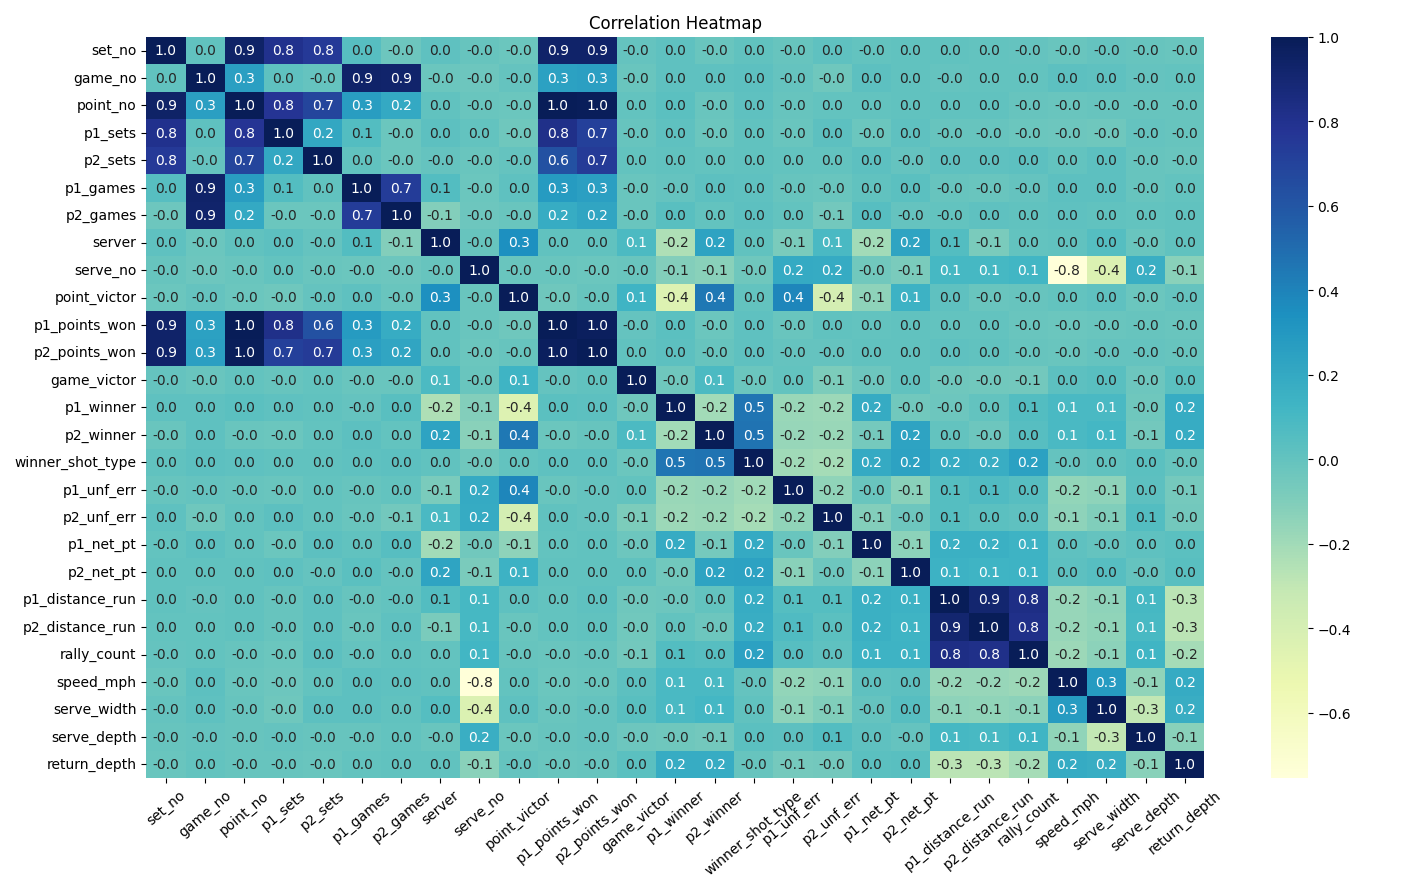
\includegraphics[width=1.05\textwidth]{figure/correlation heatmap.png}
     % \vspace{-0.3cm}
    \caption{Correlation Heatmap Based on Spearman Correlation Analysis
    \textnormal{}}
    \label{fig:correlation_heatmap }
    % \vspace{-0.5cm}
\end{figure}

According to the correlation heatmap, the correlation coefficients between the distance run by the two players in the match ("p1\_distance\_run", "p2\_distance\_run") and the number of strokes in the match ("rally\_count") are $\geq 0.8$, which indicates that there is a strong correlation between them. It can be understood that the more the number of hits in the game, the longer the distance run in the game, so we only keep the number of hits in the game ("rally\_count") field, and delete the distance run by the two players in the game ("p1\_distance\_run", "p2\_distance\_run"), so as to achieve the effect of the data dimensionality reduction. Based on this kind of correlation analysis, we did dimensionality reduction on the data, extracted some fields that are more independent from each other, and finally extracted 27 fields for subsequent model training.




\subsection{Model Structure}\label{sec:model_structure}
On a real field of play, the game situation has the following insight into the impact of the game on the player: the closer the point is to the current game, the greater the impact on the player.\cite{insight} Therefore, to simulate this effect, we modeled a long and short-term memory network based model to capture the flow of points occurring while the game is in progress.


Long Short-Term Memory (LSTM) is a special kind of Recurrent Neural Network (RNN), widely used in the field of Natural Language Processing.The core idea of LSTM is its so-called "Cell state" and its interaction with three gate controllers: Input Gate, Forget Gate, Output Gate. During the training process, the network learns the parameters of these three gate controllers dynamically. Through the collaboration of the three gates, the LSTM can selectively remember or forget information, and therefore can efficiently process sequences of different lengths. Figure \ref{fig:lstm_struction} shows the exact structure of the LSTM model we built.

\begin{figure}[htbp]
    \centering
    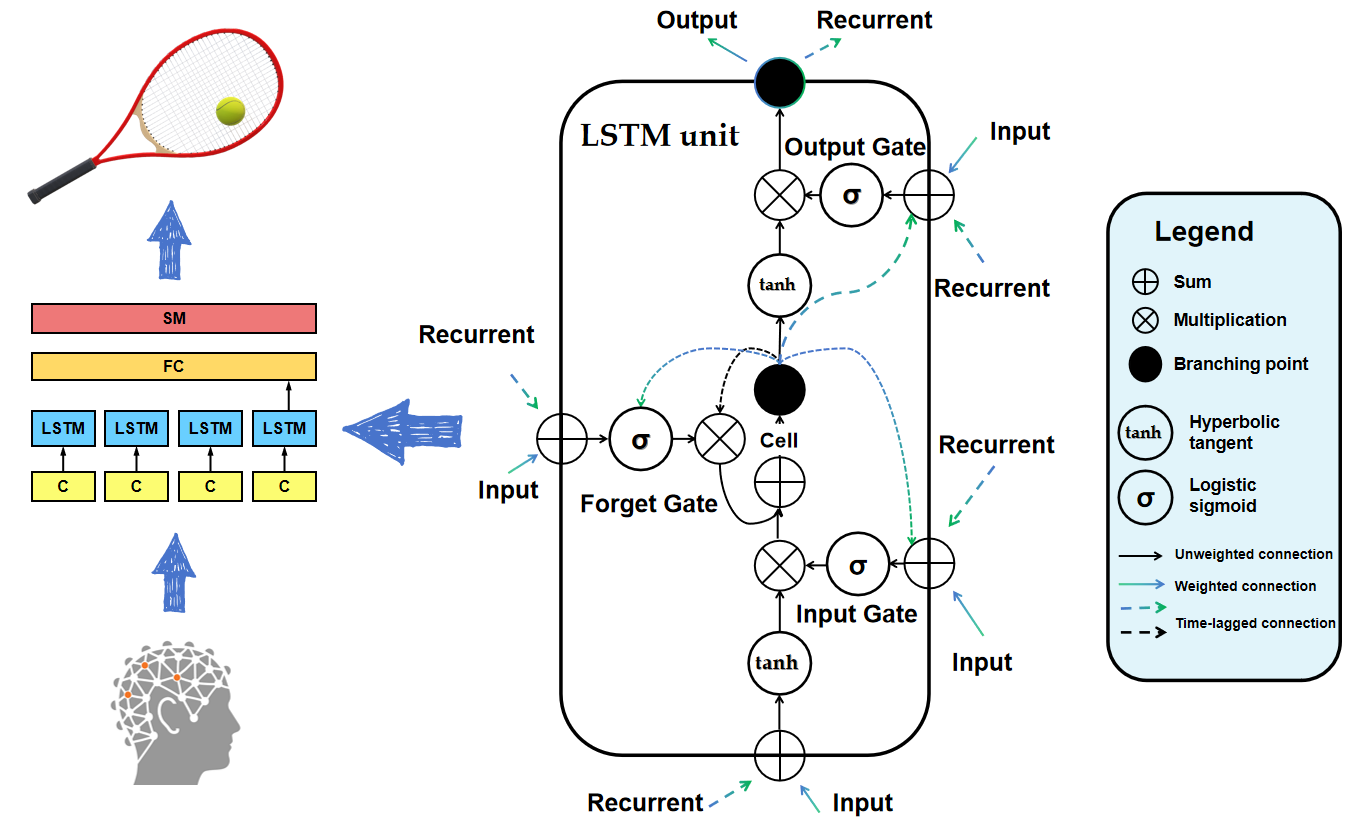
\includegraphics[width=0.9\textwidth]{figure/lstm_structure.png}
    % \vspace{-0.3cm}
    \caption{The Structure Diagram of LSTM
    \textnormal{}}
    \label{fig:lstm_struction}
    % \vspace{-0.5cm}
\end{figure}

We employ LSTM to simulate players' behavior during a match. In this simulation, the Cell state in LSTM represents the player's current match status, the Input Gate simulates the player's reception of current changes on the field, the Forget Gate simulates the player's forgetting of previous match conditions, and the Output Gate simulates the actions taken by the player based on the current match status. Additionally, we construct a sequence of dimensionally reduced point data from a match, which serves as the input to the model and is denoted as $x_t$ . Specifically:


\begin{itemize}[label=\textbf{\normalsize$\bullet$}]
    \item Input Gate determine what new information will be added to the unit state, similar to how an player adjusts his or her tactics and techniques in a game based on the current round and the opponent's strategy. We denote the input gate as $I_t$. The expression of $I_t$ is:
    % 这是输入门的变量取值
    \begin{equation}I_{t}=\sigma(x_{t}\cdot k_{1}+h_{t-1}\cdot k_{2}+b_{1})\end{equation}

    \item Forget Gate determines which information in the unit state should be discarded, similar to how an player ignores or forgets the favorable and unfavorable factors of previous rounds in a game in order to focus on the current challenge. In the current match, information that is further away from the present is more likely to be discarded by the oblivion gate, and their impact on the current situation gradually diminishes. This is similar to the human brain's forgetting curve. We denote the forget gate as $F_t$. The expression of $F_t$ is:
    % 这是遗忘门的变量取值
    \begin{equation}F_{t}=\sigma(x_{t}\cdot k_{3}+h_{t-1}\cdot k_{4}+b_{2})\end{equation}
    \item Output Gate determine which parts of the unit's state will be used to generate the current output, similar to how an player decides their next move based on the current round and previous experience. We denote the output gate as $O_t$. The expression of $O_t$ is:
    % 这是输出门的变量取值
    \begin{equation}O_{t}=\sigma(x_{t}\cdot k_{5}+h_{t-1}\cdot k_{6}+b_{3})\end{equation}
    \end{itemize}
    
During the training process, the Cell state is updated based on the Input Gate and Forget Gate, after which the Output Gate forms the output based on the value of the Cell state.
% \begin{figure}[htbp]
%     \centering
%     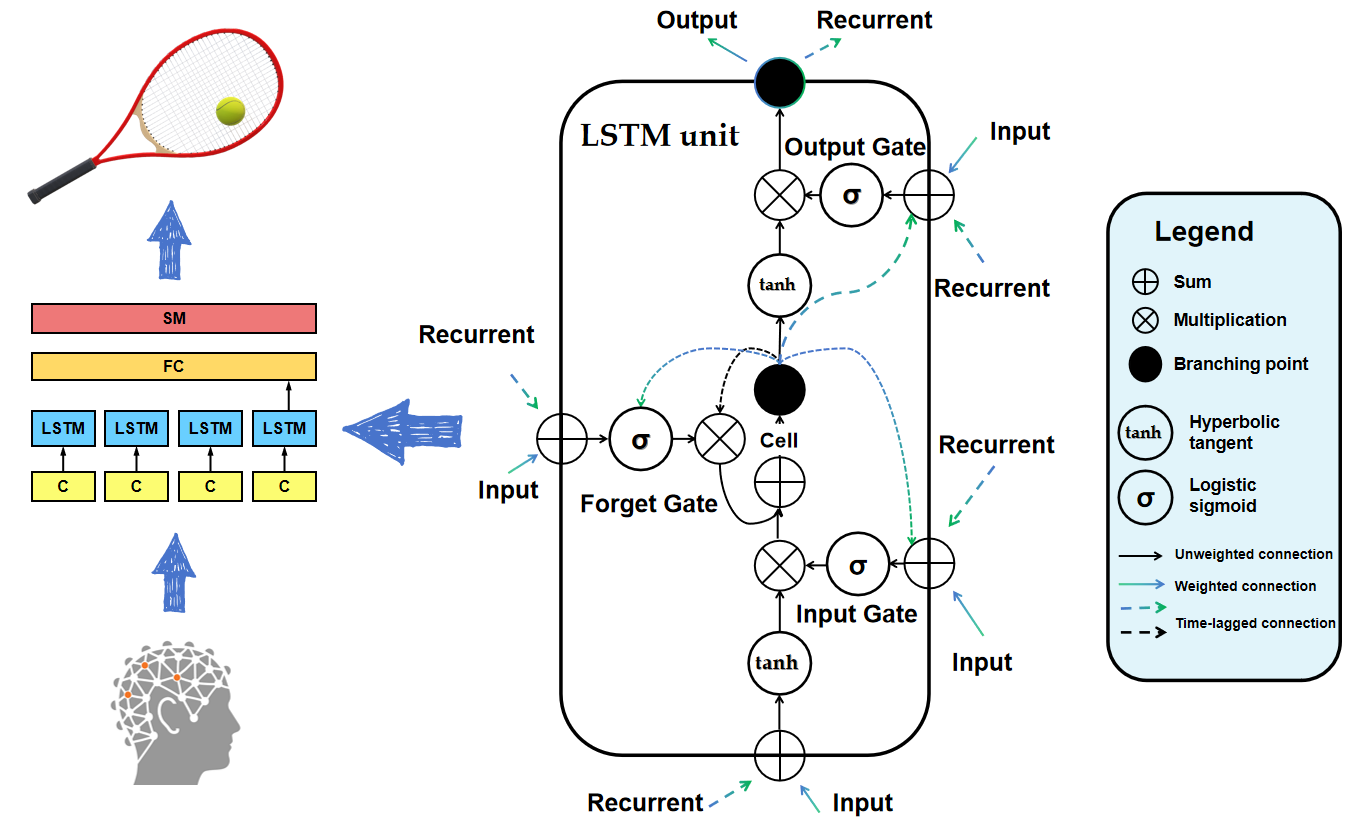
\includegraphics[width=0.9\textwidth]{figure/lstm_structure.png}
%     % \vspace{-0.3cm}
%     \caption{The structure diagram of LSTM
%     \textnormal{}}
%     \label{fig:lstm_struction}
%     % \vspace{-0.5cm}
% \end{figure}

\subsection{Training and Predicting Results}
We utilize the dataset provided by MCM, allocating \(90\%\) of the data for model training and the remaining \(10\%\) for testing. After iterating through 1000 training epochs, the model's loss function values are presented in Figure \ref{fig:lstm_loss}. The results indicate that our model achieves an accuracy rate of \(94.52\%\) on unseen data, demonstrating its robust generalization capabilities to accurately predict players' scores in real match scenarios.

% \vspace*{-10pt}
\begin{figure}[htbp]
  \centering
  \subfigure[Training Loss]{%
    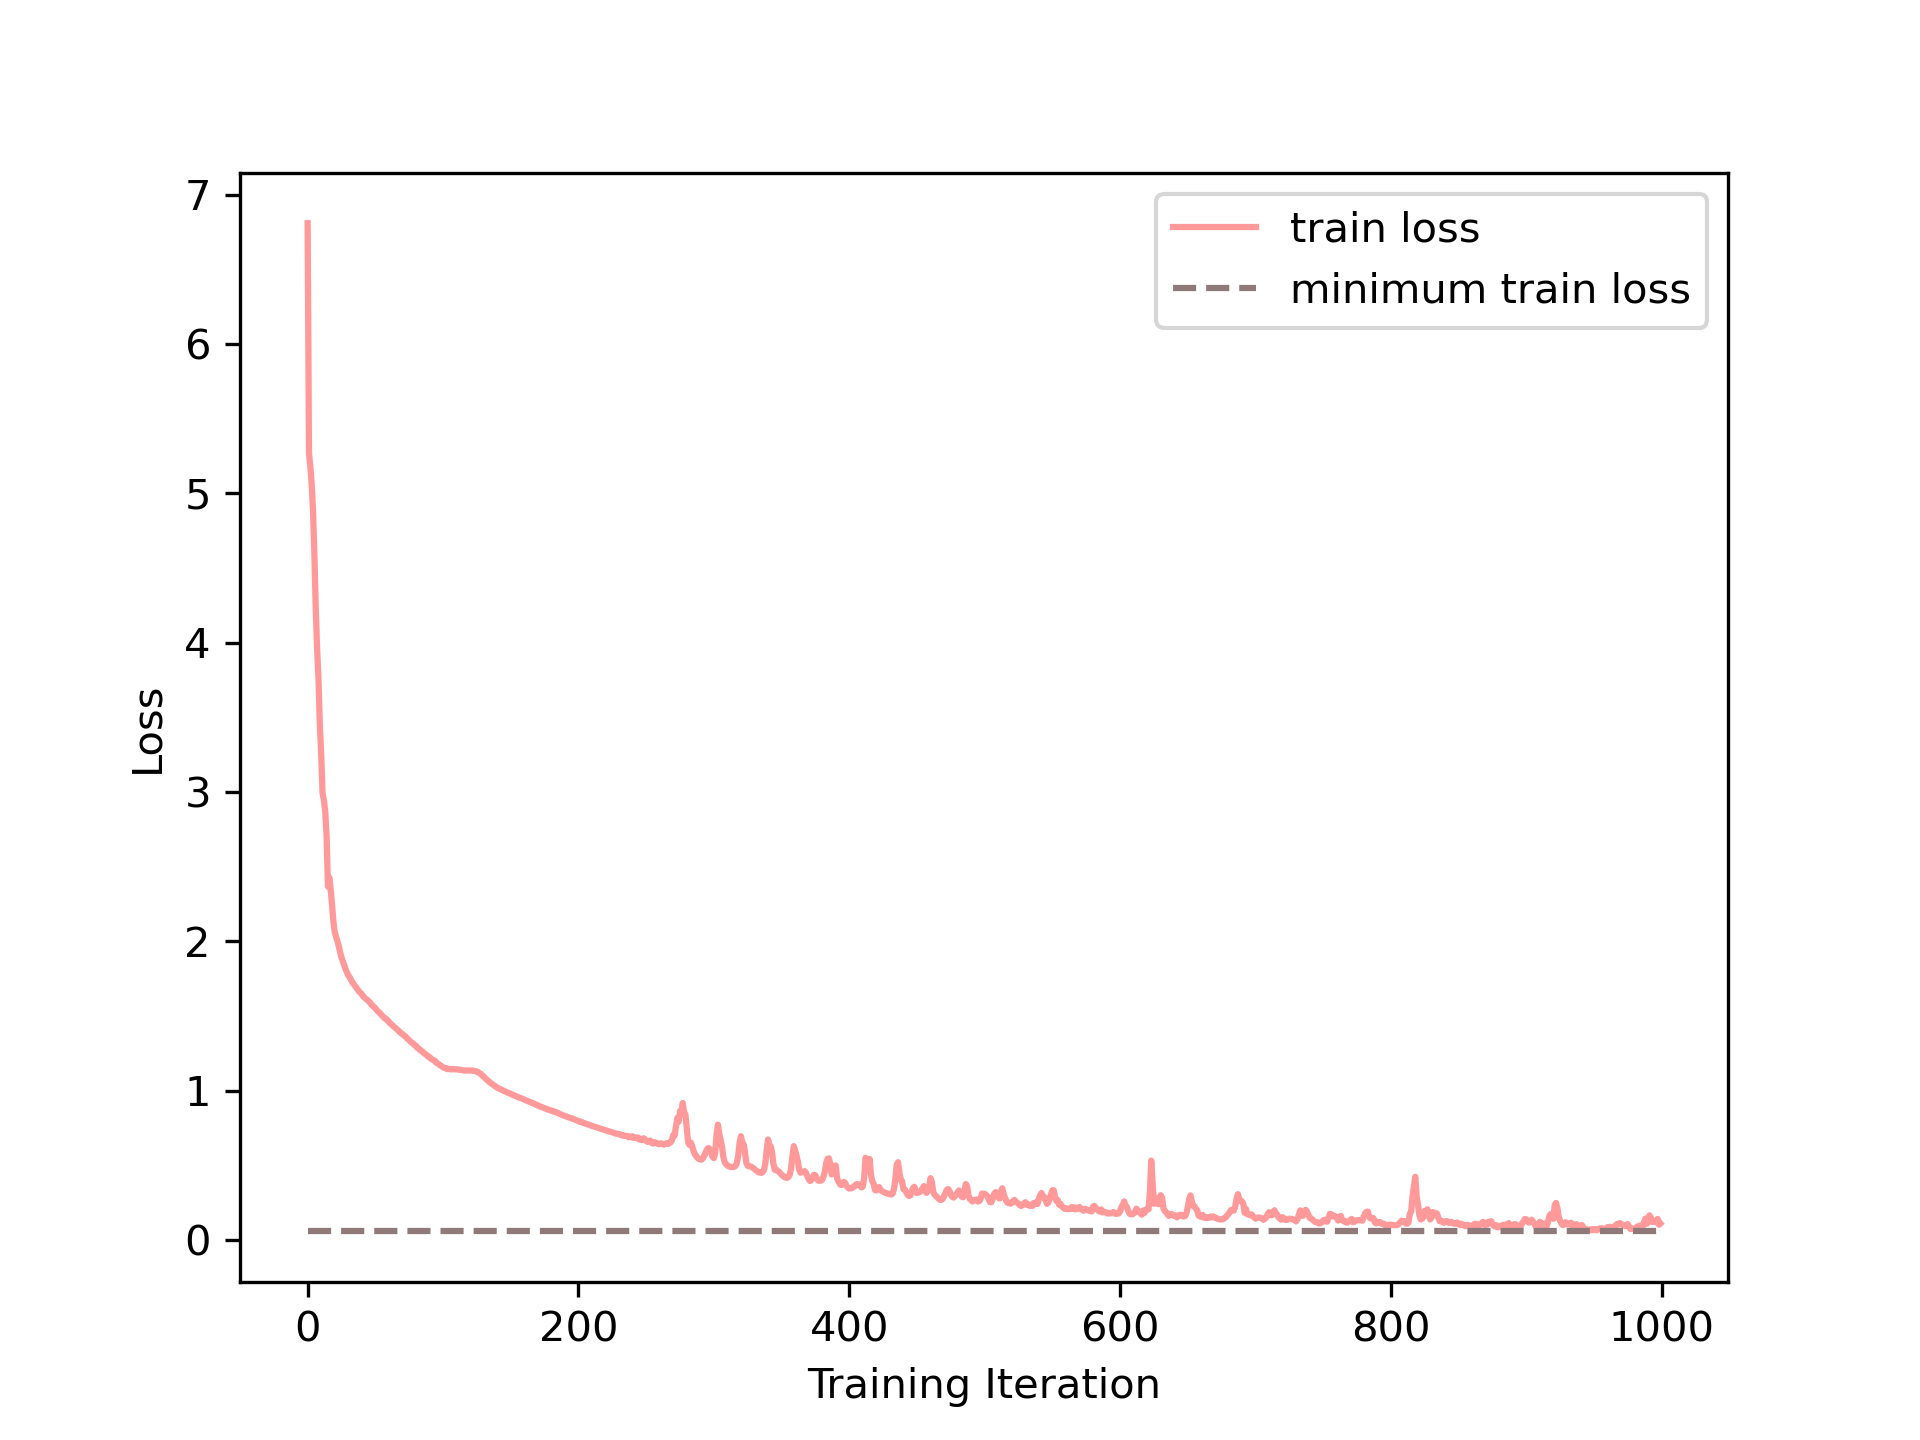
\includegraphics[width=0.48\textwidth]{figure/loss_curve_lstm_train.png}
    \label{fig:train_loss}
  }
  \subfigure[Testing Loss]{%
    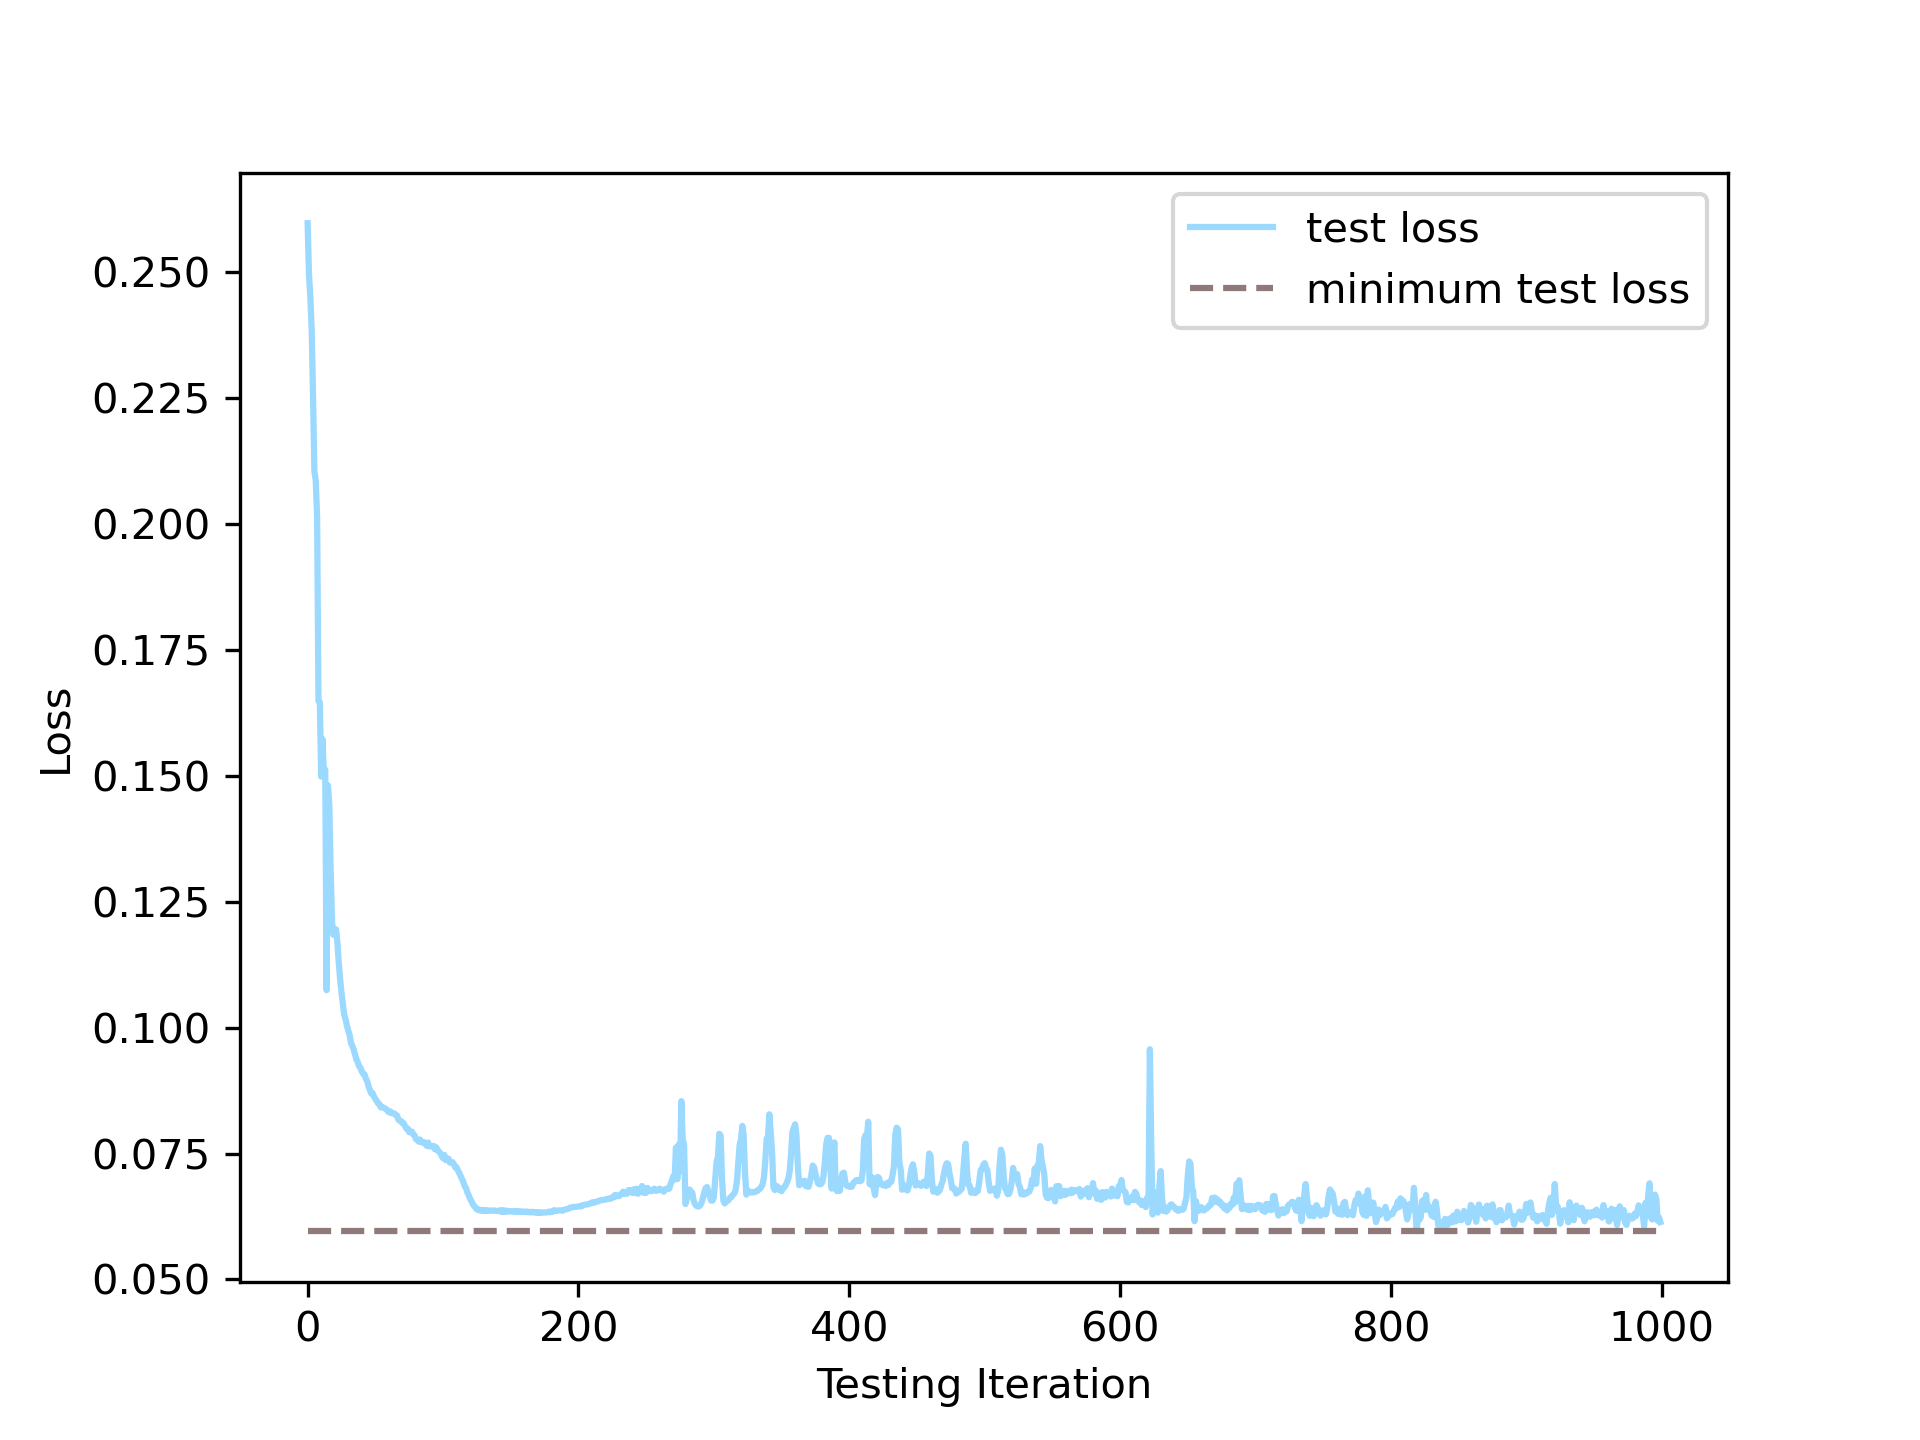
\includegraphics[width=0.48\textwidth]{figure/loss_curve_lstm_test.png}
    \label{fig:test_loss}
  }
  \caption{The Loss Curve for MM-LSTM}
  \label{fig:lstm_loss}
\end{figure}

Based on this, we visualized the match process between Carlos Alcaraz and Novak Djokovic (whose data was not used for training) as shown in Figure \ref{fig:match_visual}. The X-axis represents the flow of the match, with the blue section representing Carlos Alcaraz and the green section representing Novak Djokovic. We used the area of the bar chart to represent the performance score of the player at the current moment, with both players’ performance scores ranging between 0 and 1, summing up to 1. The player with the higher performance score at each moment is predicted to be the winner of the game.

\begin{figure}[htbp]
    \centering
    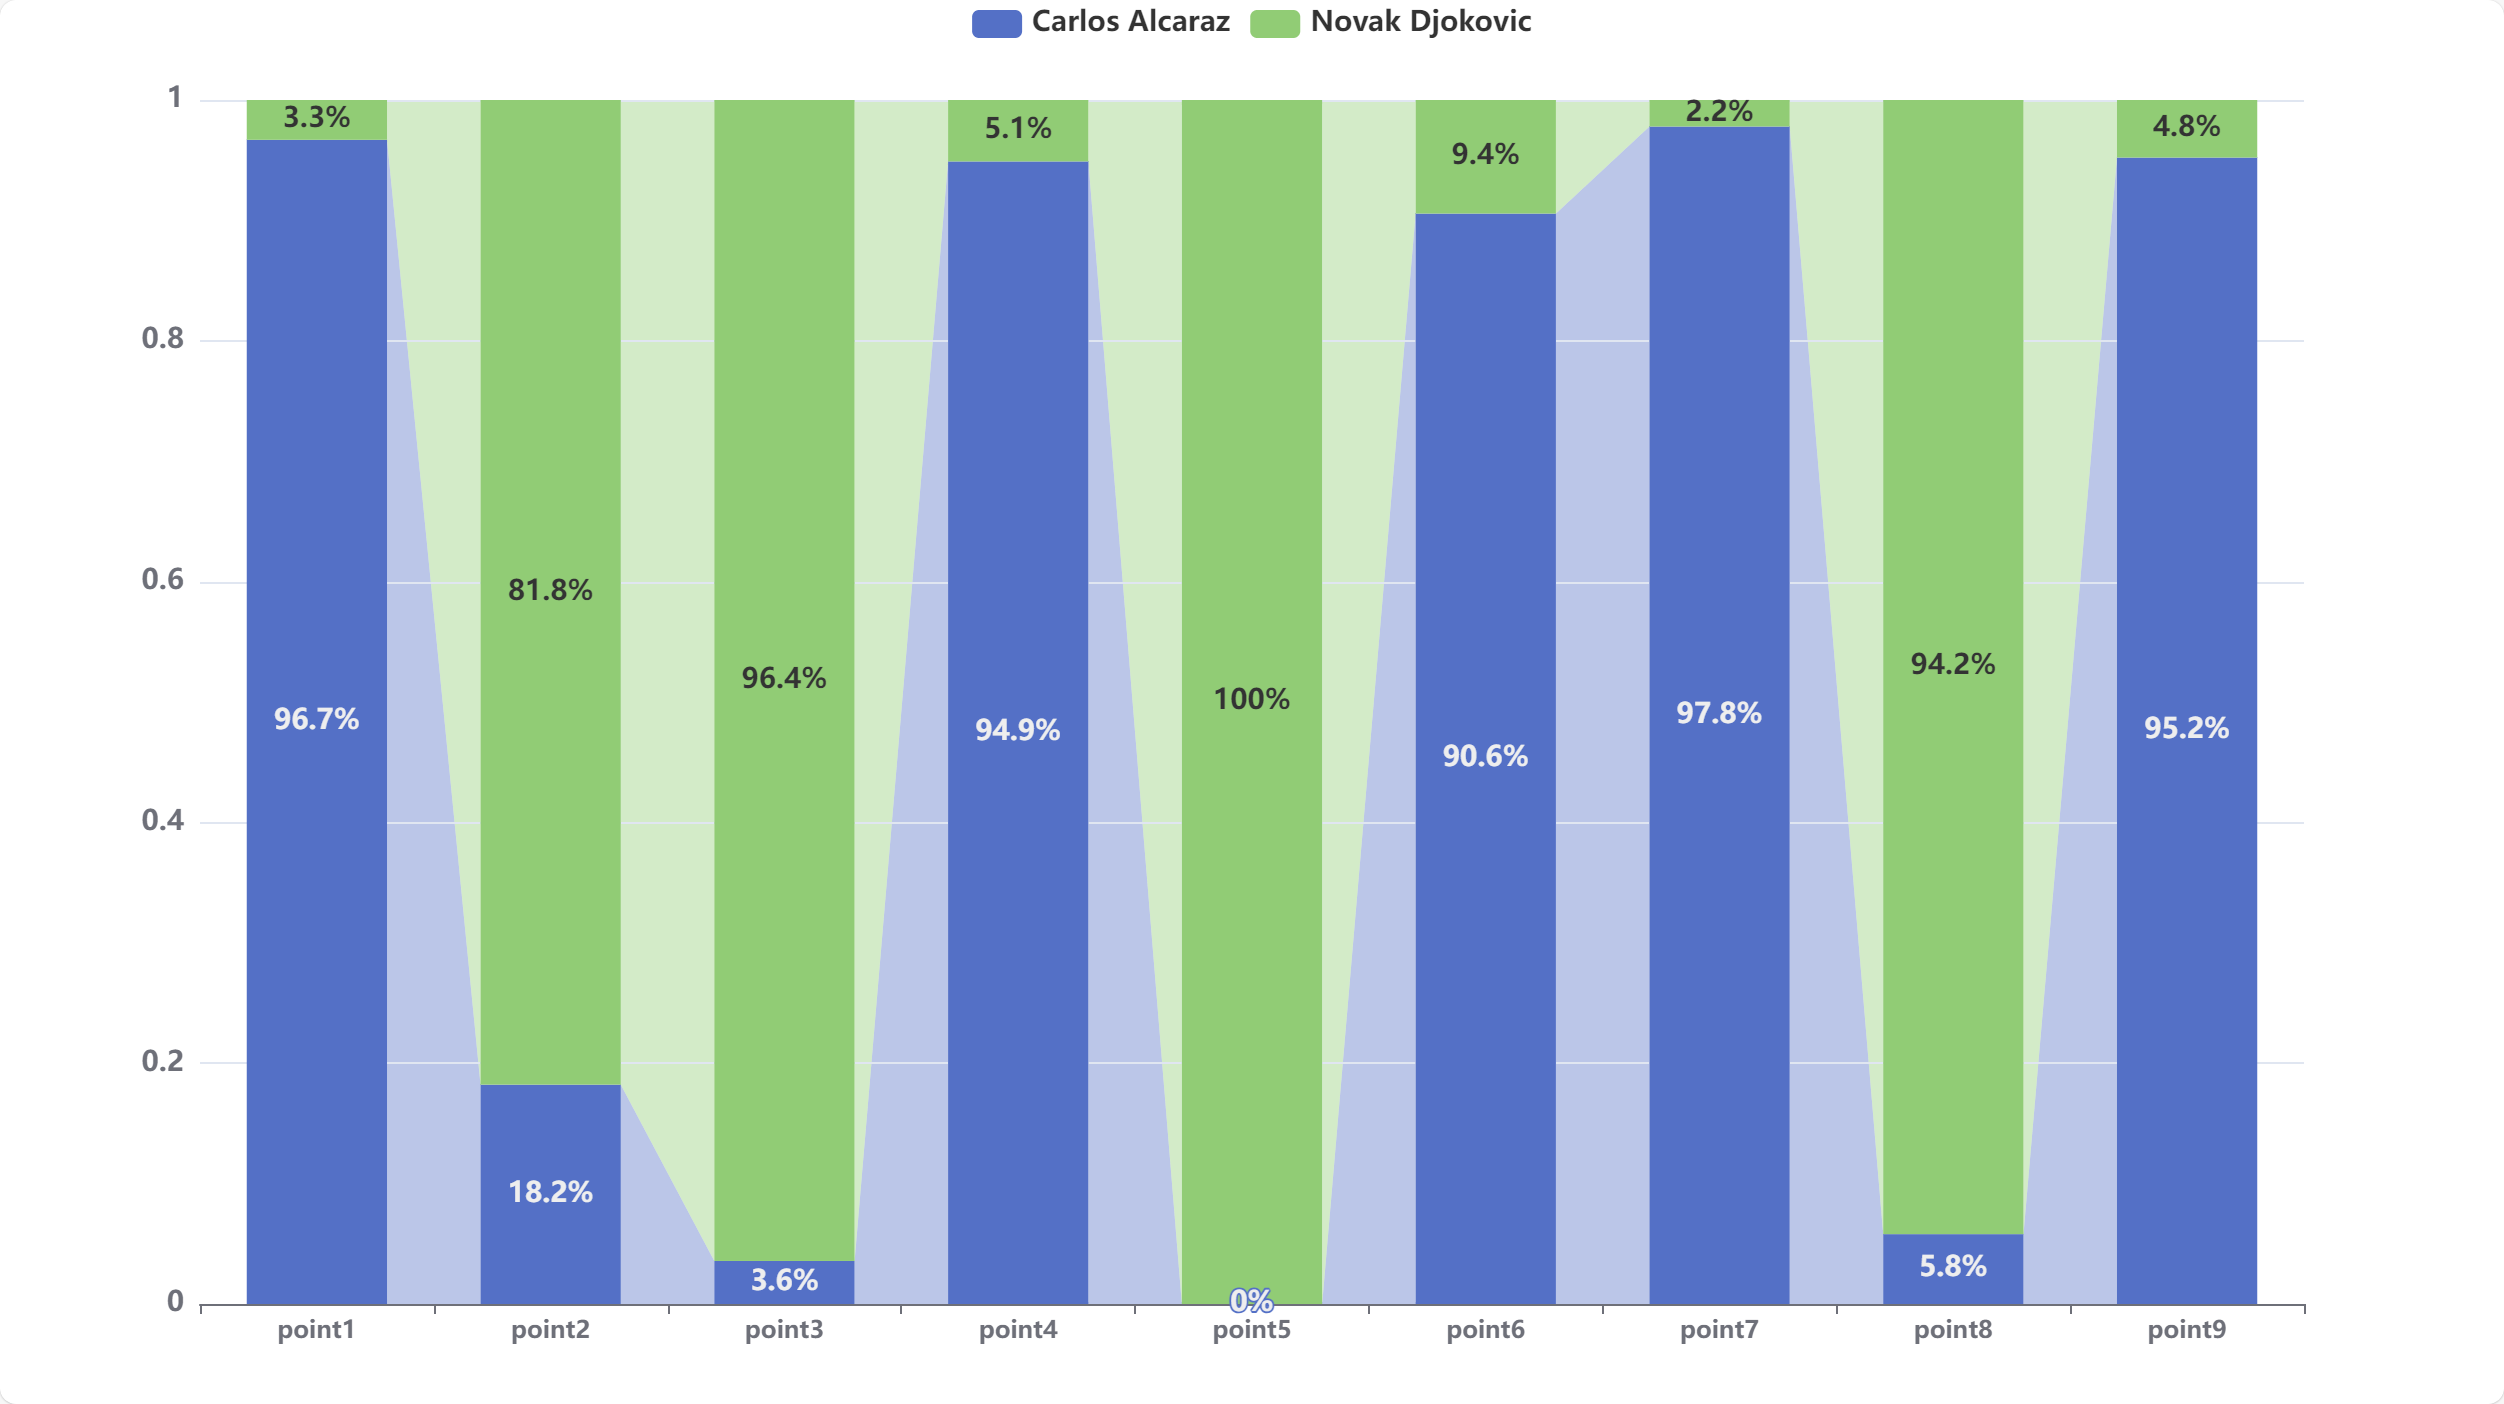
\includegraphics[width=0.95\textwidth]{figure/match_visual.png}
    % \vspace{-0.3cm}
    \caption{Match Flow Visualization: Carlos Alcaraz vs. Novak Djokovic
    \textnormal{}}
    \label{fig:match_visual}
    % \vspace{-0.5cm}
\end{figure}

% \subsection{Momentum-based LSTM Model Representation}
% To illustrate the correlation between our LSTM model and momentum, we simplify the modeled LSTM model into a well-formed momentum model based on the following equations.

% % The traditional momentum model is formulated as follows:
% % \begin{equation}
% % \begin{aligned}
% % p_* & =\sum p_i \\
% % & =\sum m_i v_i
% % \end{aligned}
% % \end{equation}

% Our LSTM model is formulated as follows, Our LSTM model is formulated as follows, where $I_t$, $F_t$, $O_t$, $C_t$ represent the input gate, forget gate, output gate, Cell state mentioned in Section 3.2, respectively:
% \begin{equation}
% \begin{gathered}
%     H_{t} = O_{t} \cdot \tanh(C_{t}) = O_{t} \cdot \tanh\left(F_{t} \cdot C_{t-1} + I_{t} \cdot \tilde C_{t}\right) \label{eq:lstm_base}
% \end{gathered}
% \end{equation}

% Based on the formula for input gate, forget gate, output gate mentioned in \ref{sec:model_structure}, we can expand the formula \ref{eq:lstm_base}:
% \begin{equation}
% \begin{gathered}
%     H_{t} = \sigma(x_{t} \cdot k_{5} + h_{t-1} \cdot k_{6} + b_{3}) \cdot \tanh\left(\sigma(x_{t} \cdot k_{3} + h_{t-1} \cdot k_{4} + b_{2}) \cdot C_{t-1} \right.\\
%     \quad \left. + \sigma(x_{t} \cdot k_{1} + h_{t-1} \cdot k_{2} + b_{1}) \cdot \tanh\left(x_{t} \cdot k_{7} + h_{t-1} \cdot k_{8} + b_{4}\right)\right)\label{eq:lstm_expand}
% \end{gathered}
% \end{equation}

% Simplify the formula \ref{eq:lstm_expand}:
% \begin{equation}
% f_{i}(x_{t}) = x_{t}\cdot k_{a_{i}(t)} + h_{t-1} \cdot k_{b_{i}(t)} + b_{c_{i}(t)}
% \end{equation}
% % 这是使用f代替后的表达式
% \begin{equation}H_{t} = \sigma\left( f_{1}(x_{t}) \right) \cdot \tanh\left( \sigma(f_{2}(x_{t})) \cdot C_{t-1} + \sigma(f_{3}(x_{t})) \cdot \tanh(f_{4}(x_{t})) \right)\label{eq:lstm_simply}
% \end{equation}

% We extract a part of the formula \ref{eq:lstm_simply}, denoted $P_n$:

% % 三个公式全都对齐
% % \begin{equation}\begin{aligned}P_n&=\sigma(f_2(x_t))\cdot C_{t-1}+\sigma(f_3(x_t))\cdot\tanh(f_4(x_t)))\\&=F_2(x_t)C_{t-1}+F_3(X_t)\cdot\tanh(f_4(X_t))\\&=A+B\cdot\tan h(F_4(x_t))\\&=A+\alpha(p)\\
% % A&=F_2(x_t)C_{t-1}+F_3(X_t)\\B&=F_3(x_t)\end{aligned}\end{equation}

% % 三个公式不对齐
% % \begin{equation}\begin{aligned}P_n&=\sigma(f_2(x_t))\cdot C_{t-1}+\sigma(f_3(x_t))\cdot\tanh(f_4(x_t)))\\&=F_2(x_t)C_{t-1}+F_3(X_t)\cdot\tanh(f_4(X_t))\\&=A+B\cdot\tan h(F_4(x_t))\\&=A+\alpha(p)\end{aligned}\end{equation}
% \begin{equation}\begin{aligned}P_n&=\sigma(f_2(x_t))\cdot C_{t-1}+\sigma(f_3(x_t))\cdot\tanh(f_4(x_t)))\\&=F_2(x_t)C_{t-1}+F_3(X_t)\cdot\tanh(f_4(X_t))\end{aligned}\end{equation}


% Then we simply Pn:
% % \begin{equation}A=F_2(x_t)C_{t-1}+F_3(X_t)\end{equation}
% % \begin{equation}B=F_3(x_t)\end{equation}
% % \begin{equation}P_n=A+B\cdot\tanh(F_4(x_t))=A+\alpha(p)\end{equation}
% % \begin{equation}\begin{aligned}P_n&=A+B\cdot\tanh(F_4(x_t))\\&=A+\alpha(p)\end{aligned}\end{equation}
% % \begin{equation}\begin{aligned}P_n&=\sigma(f_2(x_t))\cdot C_{t-1}+\sigma(f_3(x_t))\cdot\tanh(f_4(x_t)))\\&=F_2(x_t)C_{t-1}+F_3(X_t)\cdot\tanh(f_4(X_t))\\&=A+B\cdot\tanh(F_4(x_t))\\&=A+\alpha(p)\end{aligned}\end{equation}

% \begin{equation}
% \left\{
% \begin{aligned}
%     A &= F_2(x_t)C_{t-1}+F_3(X_t) \\
%     B &= F_3(x_t) \\
%     P_n &= A+B\cdot\tanh(F_4(x_t)) \\
%     &= A+\alpha(p)
% \end{aligned}
% \right.
% \end{equation}

% Thus, We can divide the formula in \ref{eq:lstm_simply} into two parts, $F_1$, $P_n$. $F_1$ denotes the function of the race at the current point in time, and Pn denotes the temporal part, which includes the content of the cell state in the LSTM, i.e., the effect of the previous race situation on the athlete.
% \begin{equation}F_{1}(x_t)=\sigma(f_1(x_{t}))\end{equation}
% \begin{equation}P_n=A+\alpha(p)\\\end{equation}
% \begin{equation}H_{t}=F_1(x_{t})\cdot\tanh(P_{n})\end{equation}

% % \begin{equation}
% % \left\{
% % \begin{aligned}
% %     F_{1}(x_t) &= \sigma(f_1(x_{t})) \\
% %     P_n &= A+\alpha(p) \\
% %     H_{t} &= F_1(x_{t})\cdot\tanh(P_{n})
% % \end{aligned}
% % \right.
% % \end{equation}
% The $\alpha(p)$ in the timing part $P_n$ represents the effect of momentum on the player during the match. This momentum consists of two components: one is the hard power of the player, and the other is the soft power of the player (e.g., scoring, the effect of the opponent on the player's mood during the match, etc.).


                                
% \subsection{Figures}

% \begin{figure}[h]
%     \centering
%     \includegraphics[width=0.7\linewidth]{figure/comap_logo}
%     \caption{Comap logo}
%     \label{fig:comap-logo}
% \end{figure}
% \begin{algorithm}
%     \caption{LSTM Computation}
%     \label{algorithm:lstm}
%     \SetAlgoNlRelativeSize{-1}
%     \SetAlgoNlRelativeSize{-2}
%     \SetAlgoNlRelativeSize{-1}
%     \KwIn{Input data $x_t$, previous hidden state $h_{t-1}$, parameters $k_1, k_2, \ldots, k_8$, and biases $b_1, b_2, \ldots, b_4$}
%     \KwOut{Current hidden state $h_t$}
    
%     // Forget gate\;
%     $I_t \gets \sigma(x_t \cdot k_1 + h_{t-1} \cdot k_2 + b_1)$\;

%     // Output gate\;
%     $F_t \gets \sigma(x_t \cdot k_3 + h_{t-1} \cdot k_4 + b_2)$\;

%     // Candidate memory state\;
%     $\tilde{c}_t \gets \tanh(x_t \cdot k_7 + h_{t-1} \cdot k_8 + b_4)$\;

%     // Update memory state\;
%     $C_t \gets F_t \cdot C_{t-1} + I_t \cdot \tilde{c}_t$\;

%     // Output hidden state\;
%     $O_t \gets \sigma(x_t \cdot k_5 + h_{t-1} \cdot k_6 + b_3)$\;

%     // Compute current hidden state\;
%     $h_t \gets O_t \cdot \tanh(C_t)$\;

%     \KwRet{$h_t$}\;
% \end{algorithm}

% \begin{algorithm}
%     \caption{Combined LSTM Expression}
%     \label{algorithm:lstm-expression}
%     \SetAlgoNlRelativeSize{-1}
%     \SetAlgoNlRelativeSize{-2}
%     \SetAlgoNlRelativeSize{-1}
%     \KwIn{Input data $x_t$, previous hidden state $h_{t-1}$, parameters $k_1, k_2, \ldots, k_8$, and biases $b_1, b_2, \ldots, b_4$}
%     \KwOut{Current hidden state $H_t$}
    
%     // Use substitute functions $f_i(x_t)$\;
%     $f_1(x_t) \gets x_t \cdot k_5 + h_{t-1} \cdot k_6 + b_3$\;
%     $f_2(x_t) \gets x_t \cdot k_3 + h_{t-1} \cdot k_4 + b_2$\;
%     $f_3(x_t) \gets x_t \cdot k_1 + h_{t-1} \cdot k_2 + b_1$\;
%     $f_4(x_t) \gets x_t \cdot k_7 + h_{t-1} \cdot k_8 + b_4$\;

%     // Compute hidden state\;
%     $H_t \gets \sigma(f_1(x_t)) \cdot \tanh(\sigma(f_2(x_t)) \cdot C_{t-1} + \sigma(f_3(x_t)) \cdot \tanh(f_4(x_t)))$\;

%     \KwRet{$H_t$}\;
% \end{algorithm}


\section{Problem 2: Momentum Modeling and Evaluation of Long Short-Term Memory Networks (MM-LSTM)}

\subsection{Stochastic Probability Based Winner Prediction}

In order to assess whether momentum plays any role in the match, we first develop a stochastic probability-based prediction model of winning percentage. We choose three empirical metrics to parameterize this stochastic probability model:
\begin{itemize}[label=\textbf{\normalsize$\bullet$}]
    \item $P_{base}$: the win rate value of a player base, set to a fixed value of 0.5.
    \item $P_{server}$: the portion of a player's win rate that is increased over the base win rate as a server.
    \item $m_i$: the strength value of $player_i$.
    \item $P_{factors}$:the probability change value caused by factors.
\end{itemize}

The computation of $P_{server}$ and $m_i$ is described below in turn:

For $P_{server}$, we analyzed the win rates of players as servers based on the data set of Wimbledon 2023 Gentlemen's singles matches after the second round provided by MCM. It was found that the probability of winning as a server decreases over the different sets of a match, suggesting that the effect of the serve on a player's win decreases as the match progresses. Also based on the analysis of the paper by researchers at the University of Amsterdam \cite{p_server}, we integrate both and decide to only consider the impact of the serving position in the first two games.

We have done a statistical analysis of the probability of a server winning in the data set, and the base value of the increase in the probability of a player winning by serving is 0.173119165. Based on this, we modeled the $P_{server}$ formulation as follows:

% % 描述先决条件中基础概率与发球手位置增加的概率
% \begin{equation}
% R_{server}=0.173119165
% \end{equation}
% % 在这里指出发球位置对于胜利的影响
% \[ P_{server} = \left\{
% \begin{array}{ll}
% 2 \cdot R_{server}, & \text{set\_no} = 1 \\
% R_{server}, & \text{set\_no} = 2 \\
% 0, & \text{set\_no} > 2
% \end{array}
% \right.
% \]

\begin{equation}
R_{server}=0.173119165
\end{equation}
\begin{equation}\left.P_{server}=\left\{\begin{array}{ll}2\cdot R_{server},&\text{set\_no}=1\\R_{server},&\text{set\_no}=2\\0,&\text{set\_no}>2\end{array}\right.\right.\end{equation}

Similarly, for other factors, we also use similar methods for analysis, and ultimately use the following formula to calculate:
\begin{equation}
 \sum P_{factors} = P_{server} + \sum P_{others} 
\end{equation}

For $m_i$, we take the ratio of the final scores and other factors of two players in a game as the relative ratio of their strengths, based on which we calculate the strength intensity of each player as the value of $m_i$. The specific steps are as follows:


\begin{enumerate}
  \item Initialize the player list, set two attributes for each player: relative\_strength, strength\_ratio. relative\_strength is a list of the relative strength of the players, set its initial value to 100; strength\_ratio Indicates the relative ratio of strength between the player as player1 and the corresponding player2.
  \item Iterate through Wimbledon\_featured\_matches.csv, get the player1, player2, p1\_point\_won and p2\_point\_won at the end of each match. For each player1, the value of p1\_point\_won divided by p2\_point\_won is recorded in strength\_ratio as its strength relative to player2.
  \item Iterate through the list of players and get the relative\_strength of the current player, recorded as player1\_strength. Calculate the player2\_strength of the corresponding player2, whose value is equal to player1\_strength * ratio. After that, add the calculated play2\_strength to the relative\_strength list of player2.
  \item Iterate through the list of players, and if the player's relative\_strength has more than one value, take the average of the values and use it as the new relative\_strength.
  \item Scales the relative\_strength of each player to a value between 0 and 100.
\end{enumerate}

% The pseudo-code description of the above process is shown in Algorithm \ref{algo:player_strength}:


% \begin{algorithm}
% \footnotesize
% 	\caption{Calculation of Player Strength Value $S_i$}
% 	\label{algo:player_strength}
% 	\begin{algorithmic}[1]
% 		\Require Competition data $D_f$
% 		\Ensure Relative strength of players in k matches $S = \{S_1, S_2, \dots , S_k\}$
%         \Function{$GetStrengthRatios$}{$D_f$}:
% 			\For{each $Match_i$ of $D_f.Matchs$}
%                     \If{$Match_i \in D_f.Player.Type$}
%                         \State $Ratios \gets $ $\frac{Match_i.Point[0]}{Match_i.Point[1]}$
%                     \EndIf
%                 \EndFor
% 		      \State \Return $Ratios$
% 		\EndFunction\\
    
%         \Function{$GenerateStrengthRatios$}{$Ratio_i, Players$}:
% 			\State $Strength \gets Initialization()$
%                 \For{$Player \text{ of } Players$}
%                     \If{$Ratios\_i.label \in Player.name$}
%                 \State $Strength \gets Ratios\_i.data \times Player.Ratio$
%             \EndIf
%         \EndFor
%         \State \Return $Strength$
% 		\EndFunction\\
  
% 		\State $StrengthRatios \gets  GetStrengthRatios(D_f)$
%         \For{each $D_{f_i}$ of $D_f$}
%             \State $Players \gets  D_{f_i}.Player1 , D_{f_i}.Player2$
%             \For{each $Ratio_i$ of $StrengthRatios$}
%                 \If{$Ratio_i \in D_f.Ratios$}
%                     \State $S_i \gets GenerateStrengthRatios(Ratio_i, Players)$
%                 \EndIf
%             \EndFor
%         \EndFor\\

%         \State $S \gets ScoreStandardize(S)$\\
%         \Return S
% 	\end{algorithmic}
% \end{algorithm}


Based on the obtained $P_{server}$ and $m_i$ above, we model the probability of player1 winning under stochastic probability as follows:

% 在随机概率下,play1获胜的概率
\begin{equation}P_{1} = \frac{\left( P_{base} + \sum P_{factors} \right)\cdot m_{1}}{\left( P_{base} +\sum P_{factors}  \right) \cdot  m_{1} +\left( P_{base} -\sum P_{factors} \right) \cdot m_{2} } 
\end{equation}


% The traditional momentum model is formulated as follows:
% \begin{equation}
% \begin{aligned}
% p_* & =\sum p_i \\
% & =\sum m_i v_i
% \end{aligned}
% \end{equation}

\subsection{An LSTM Model is Equivalent to a Momentum-Based Model}\label{sec:momentum_lstm}
To illustrate the correlation between our LSTM model and momentum, we simplify the modeled LSTM model into a well-formed momentum model based on the following equations.

Our LSTM model is formulated as follows, where $I_t$, $F_t$, $O_t$, $C_t$ represent the input gate, forget gate, output gate, Cell state mentioned in Section \ref{sec:model_structure}, respectively:
\begin{equation}
\begin{gathered}
    H_{t} = O_{t} \cdot \tanh(C_{t}) = O_{t} \cdot \tanh\left(F_{t} \cdot C_{t-1} + I_{t} \cdot \tilde C_{t}\right) \label{eq:lstm_base}
\end{gathered}
\end{equation}

Based on the formula for input gate, forget gate, output gate mentioned in \ref{sec:model_structure}, we can expand the formula \ref{eq:lstm_base}:
\begin{equation}
\begin{gathered}
    H_{t} = \sigma(x_{t} \cdot k_{5} + h_{t-1} \cdot k_{6} + b_{3}) \cdot \tanh\left(\sigma(x_{t} \cdot k_{3} + h_{t-1} \cdot k_{4} + b_{2}) \cdot C_{t-1} \right.\\
    \quad \left. + \sigma(x_{t} \cdot k_{1} + h_{t-1} \cdot k_{2} + b_{1}) \cdot \tanh\left(x_{t} \cdot k_{7} + h_{t-1} \cdot k_{8} + b_{4}\right)\right)\label{eq:lstm_expand}
\end{gathered}
\end{equation}

Simplify the formula \ref{eq:lstm_expand}:
\begin{equation}
f_{i}(x_{t}) = x_{t}\cdot k_{a_{i}(t)} + h_{t-1} \cdot k_{b_{i}(t)} + b_{c_{i}(t)}
\end{equation}
% 这是使用f代替后的表达式
\begin{equation}H_{t} = \sigma\left( f_{1}(x_{t}) \right) \cdot \tanh\left( \sigma(f_{2}(x_{t})) \cdot C_{t-1} + \sigma(f_{3}(x_{t})) \cdot \tanh(f_{4}(x_{t})) \right)\label{eq:lstm_simply}
\end{equation}

We extract a part of the formula \ref{eq:lstm_simply}, denoted $P_n$:

% 三个公式全都对齐
% \begin{equation}\begin{aligned}P_n&=\sigma(f_2(x_t))\cdot C_{t-1}+\sigma(f_3(x_t))\cdot\tanh(f_4(x_t)))\\&=F_2(x_t)C_{t-1}+F_3(X_t)\cdot\tanh(f_4(X_t))\\&=A+B\cdot\tan h(F_4(x_t))\\&=A+\alpha(p)\\
% A&=F_2(x_t)C_{t-1}+F_3(X_t)\\B&=F_3(x_t)\end{aligned}\end{equation}

% 三个公式不对齐
% \begin{equation}\begin{aligned}P_n&=\sigma(f_2(x_t))\cdot C_{t-1}+\sigma(f_3(x_t))\cdot\tanh(f_4(x_t)))\\&=F_2(x_t)C_{t-1}+F_3(X_t)\cdot\tanh(f_4(X_t))\\&=A+B\cdot\tan h(F_4(x_t))\\&=A+\alpha(p)\end{aligned}\end{equation}
\begin{equation}\begin{aligned}P_n&=\sigma(f_2(x_t))\cdot C_{t-1}+\sigma(f_3(x_t))\cdot\tanh(f_4(x_t)))\\&=F_2(x_t)C_{t-1}+F_3(X_t)\cdot\tanh(f_4(X_t))\end{aligned}\end{equation}


Then we simply $P_n$:
% \begin{equation}A=F_2(x_t)C_{t-1}+F_3(X_t)\end{equation}
% \begin{equation}B=F_3(x_t)\end{equation}
% \begin{equation}P_n=A+B\cdot\tanh(F_4(x_t))=A+\alpha(p)\end{equation}
% \begin{equation}\begin{aligned}P_n&=A+B\cdot\tanh(F_4(x_t))\\&=A+\alpha(p)\end{aligned}\end{equation}
% \begin{equation}\begin{aligned}P_n&=\sigma(f_2(x_t))\cdot C_{t-1}+\sigma(f_3(x_t))\cdot\tanh(f_4(x_t)))\\&=F_2(x_t)C_{t-1}+F_3(X_t)\cdot\tanh(f_4(X_t))\\&=A+B\cdot\tanh(F_4(x_t))\\&=A+\alpha(p)\end{aligned}\end{equation}

\begin{equation}
\left\{
\begin{aligned}
    A &= F_2(x_t)C_{t-1}+F_3(X_t) \\
    B &= F_3(x_t) \\
    P_n &= A+B\cdot\tanh(f_4(x_t)) \\
    &= A+\alpha(p)
\end{aligned}
\right.
\end{equation}

Thus, we can divide the formula in \ref{eq:lstm_simply} into two parts, $F_1$, $P_n$. $F_1$ denotes the function of the race at the current point in time, and $P_n$ denotes the temporal part, which includes the content of the cell state in the LSTM, i.e., the effect of the previous race situation on the athlete.
\begin{equation}F_{i}(x_t)=\sigma(f_i(x_{t}))\end{equation}
\begin{equation}H_{t}=F_1(x_{t})\cdot\tanh(P_{n})\end{equation}
\begin{equation}
\label{ll}
P_n=A+\alpha(p)\\\end{equation}
% \begin{equation}
% \left\{
% \begin{aligned}
%     F_{1}(x_t) &= \sigma(f_1(x_{t})) \\
%     P_n &= A+\alpha(p) \\
%     H_{t} &= F_1(x_{t})\cdot\tanh(P_{n})
% \end{aligned}
% \right.
% \end{equation}
The $\alpha(p)$ in the timing part $P_n$ represents the effect of momentum on the player during the match. This momentum consists of two components: one is the hard power of the player, and the other is the soft power of the player (e.g., scoring, the effect of the opponent on the player's mood during the match, etc.).

At this point, we have modeled the LSTM model in Section \ref{sec:model_structure} into a momentum-based model, which we call MM-LSTM.


\subsection{Comparison of Stochastic Probability Model and Momentum-Based Model}

In order to compare the random probability model and the momentum-based model, we calculated the accuracy of these two models for point win/loss prediction on a test match separately. The mean accuracy of all match predictions is presented in Table \ref{tab:mean_acc}, and the results for individual match accuracies are illustrated in Figure \ref{fig:acc_lstm_stochastic}.

\begin{table}[h]
% \begin{table*}
	\centering
	\caption{Mean Prediction Accuracy of Models} 
        \vspace{8pt}
	\label{tab:mean_acc}
	\begin{tabular}{c|c}
		\toprule[1.5pt]
  % \specialrule{.1em}{0em}{0em} % 添加粗分割线
		Model & Mean Accuracy\\
        % \specialrule{.1em}{0em}{0em} % 添加粗分割线
		\midrule[1pt]
		Stochastic Probability Model & 67.776\% \\
		Momentum-Based LSTM Model & 94.229\% \\
% \specialrule{.1em}{0em}{0em} % 添加粗分割线
		\bottomrule[1.5pt]
	\end{tabular}
\end{table}
% \end{table*}

\begin{figure}[h]
    \centering
    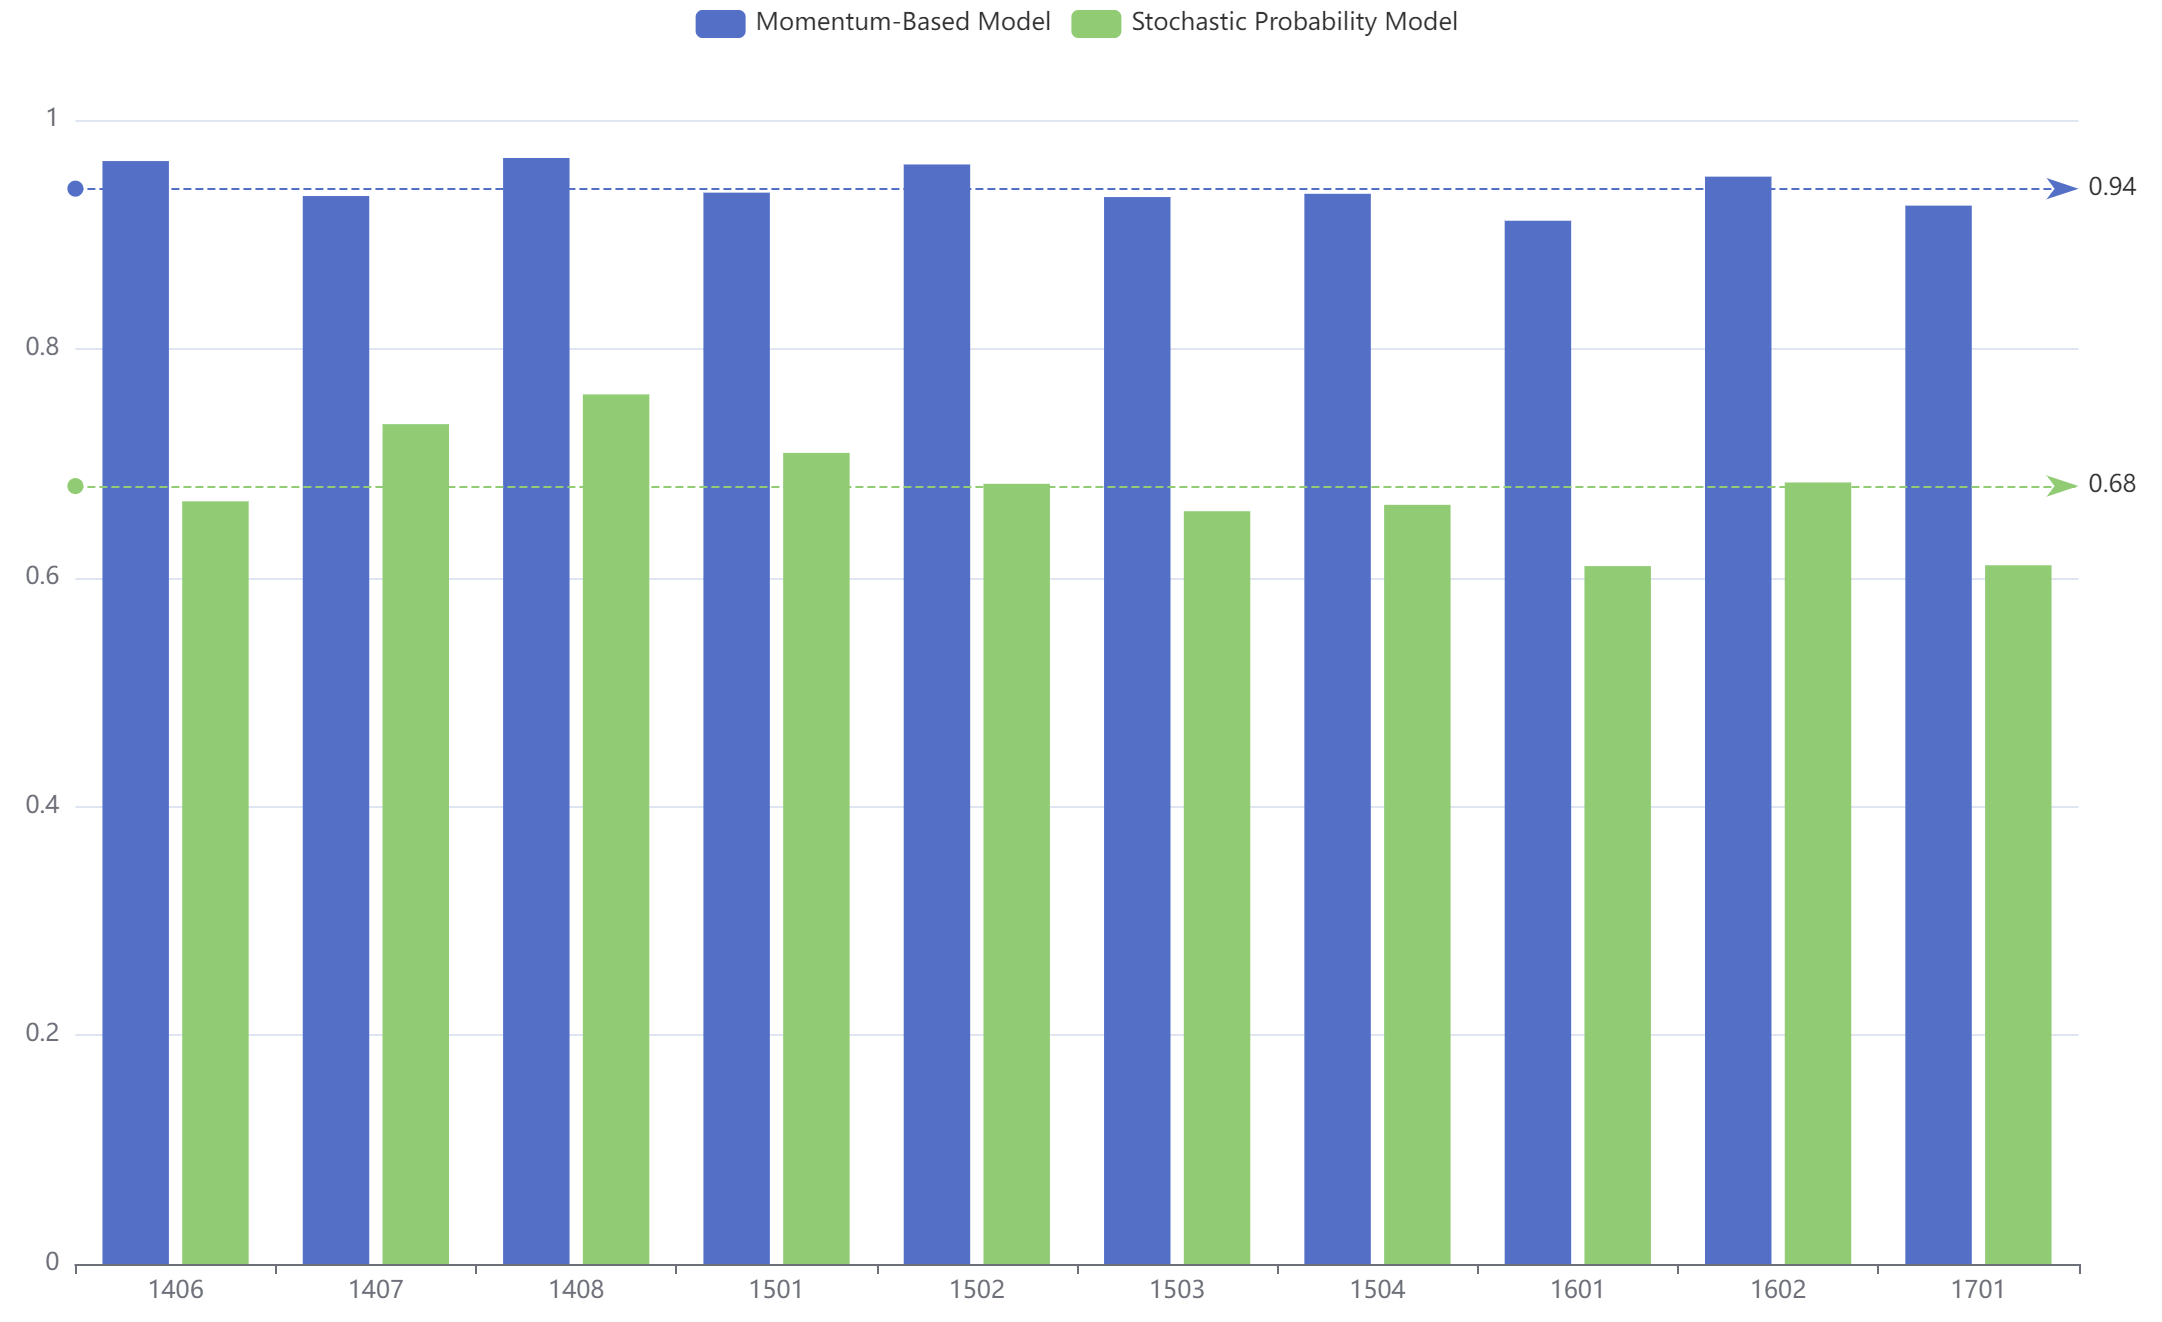
\includegraphics[width=0.8\textwidth]{figure/acc_lstm_stochastic.png}
    % \vspace{-0.3cm}
    \caption{Prediction Accuracy of Stochastic Probability Model and Momentum-Based Model 
    \textnormal{}}
    \label{fig:acc_lstm_stochastic}
    % \vspace{-0.5cm}
\end{figure}

As shown in Table \ref{tab:mean_acc}, our momentum-based model outperforms the random probability model with about 25\% accuracy. Based on this, we conclude that momentum plays a role in the game process and can be used to predict the winners and losers of the players.
\section{Problem 3: Momentum Shift Predictor Based on MM-LSTM}

\subsection{Model Structure of the Momentum Shift Predictor}\label{sec:swing_predict_model}
Based on the MM-LSTM model in Section \ref{sec:momentum_lstm}, we formulate a time-series model of the change in player scores that predicts when the situation in a match shifts from favoring one player to favoring another based on its gradient. The formula for our model is as follows:

% 描述了斜率相对差公式与动量的关系
\begin{equation}
     {K_{relative}}{(n, m)} = \frac{1}{n-m} \cdot \sum_{i=m+1}^{n} [P_i + 0.5] = \frac{1}{n-m} \cdot \sum_{i=m+1}^{n} [A+\alpha (p) + 0.5]
\end{equation}


Firstly, let's consider the score situation between two athletes, both gradually increasing over time. We assume that the functions describing these two evolving conditions are denoted as \(f_{1}\) and \(f_{2}\). Therefore, we can establish a simple mapping relationship as follows:
\begin{equation}
\left\{
\begin{aligned}
    y_{1} &= f_{1}(t) \\
    y_{2} &= f_{2}(t)
\end{aligned}
\right.
\end{equation}

In this case, we take the difference between the scores of the two athletes:
\begin{equation}
    y_1 - y_2  =  f_{1}(t) -  f_{2}(t)
\end{equation}

The gradient of their score function curves can be expressed as:
\begin{equation}
\left\{
\begin{aligned}
    % k_1 &= \frac{\delta y_{1}}{\delta t}  \\
    % k_2 &= \frac{\delta y_{2}}{\delta t}
    k_1 &= \frac{\delta y_{1}}{\delta t}  \\
    k_2 &= \frac{\delta y_{2}}{\delta t}
\end{aligned}
\right.
\end{equation}

At this point, based on our difference in scores, we can obtain a difference function whose gradient can be expressed as:
\begin{equation}
\label{ss}
    {K_{relative}}{(n, m)} = \frac{\delta (y_n - y_m)}{\delta t} = 
    \frac{\delta y_n}{\delta t} -   \frac{\delta y_m}{\delta t}
    = k_n - k_m
\end{equation}

And since the score for the nth round is determined based on the score from the (n-1)th round, the decision to score in each round relies on approximating the probability obtained from the MM-LSTM model. The probability results are rounded to obtain a binary outcome, indicating either victory (1) or failure (0). The scores are then updated based on this outcome, linking the MM-LSTM probability model with the scoring function. In another perspective, this can be viewed as a recursive formula. On this basis, we can also derive a scoring probability formula over a certain period:
\begin{equation}
    y_n = y_{n-1} + [P_n+0.5] \Longrightarrow
    y_n = y_m + \sum_{i=m+1}^{n} [P_i + 0.5] 
\end{equation}

The preceding formulas have successfully established a unified connection between probability and scores. Moving forward, let's further explore the relationship between momentum and gradient.

The following formula describes the relationship between the formula for relative gradient difference and momentum. The relative gradient difference is a metric (refer to Formula \ref{ss}) indicating score changes relative to time (or points). Here, n-m represents the variation in scores over a time period of n-m. In general, we typically set n-m to 3 (as we opted for interpolation rather than fitting). In this scenario, the score difference during this period reflects the variation in scores – the cumulative sum of whether each match results in a score. The probability P, predicted by the MM-LSTM model, approximates whether each match results in a score. Rounding P yields a binary outcome: victory (1) or failure (0). In the case of victory, points are added, causing the gradient to increase; in the event of failure, no points are added, maintaining the gradient. (Considering the relatively modest quantity of gradient, i.e., the increment in victories, over short time periods, plotting a graph with large swings may not be conducive for observation, hence the choice of a relatively large yet manageable value of 3.)

Moreover, in light of Formula \ref{ll}, where we interpret probability as momentum, we have intricately linked the relative gradient difference to momentum. Consequently, the relative gradient difference has become a key metric for analyzing changes in momentum.
\begin{equation}
\label{eq:formula25}
K_{relative}{(n, m)} = \frac{1}{n-m} \cdot \sum_{i=m+1}^{n} [P_i + 0.5] = \frac{1}{n-m} \cdot \sum_{i=m+1}^{n} [A+\alpha (p) + 0.5]
\end{equation}

The following formula represents the count of correct predictions, where \(P_i\) denotes the probability predicted at position i, representing the success probability for play 1. Applying the nested rounding function, when the prediction is successful (victory), it is rounded to 0, and when it fails (loss), it is rounded to 1. Adding 1 is done to convert the dimensional indicator of successful predictions to correspond with the dimensional indicator of \(point\_victor\). This allows for the assessment of the number of incorrect predictions. Substituting this into the frequency formula reflects the probability situation:

\begin{equation}
\label{eq:formula26}
N_{false}=\sum_{i=1}^{n}|1+[P_{i}+0.5]-Point\_victor_i|\end{equation}

The following formula is an inductive formula for calculating the final prediction accuracy:

\begin{equation}
\label{eq:formula27}
\eta_{accuracy}=\frac{N_{true}}{N_{total}}=\frac{N_{true}}{N_{true}+N_{false}} = 1-\frac{N_{false}}{N_{total}}
\end{equation}

\subsection{Factor Contribution Analysis}\label{sec:factor_contribution}
To test which factors contributed most to the model, we used a gradient importance analysis. The gradient represents the direction in which the function grows fastest at a given point, and its magnitude quantifies this maximum growth rate. For the model built in Section \ref{sec:swing_predict_model}, we calculated the partial derivative of each input with respect to the output, and then calculated the absolute value of that partial derivative and normalized it. The final normalized value obtained represents the degree of contribution of the inputs to the output.The contribution degree of some of the input indicators is shown in Table \ref{tab:gradient_importance}.

% \begin{table}[htbp]
% \centering
% \begin{tabular}{ll|ll}
% \specialrule{.1em}{0em}{0em} % 添加粗分割线
% \textbf{Factor Name} & \textbf{Value} & \textbf{Factor Name} & \textbf{Value} \\
% \specialrule{.1em}{0em}{0em} % 添加粗分割线
% point\_no & 0.0026 & serve\_no & 0.0305\\
% speed\_mph & 0.0007& game\_victor & 0.0369 \\ 
% rally\_count & 0.0319&set\_victor & 0.0282   \\ 
% server & 0.0729 & serve\_width & 0.0018 \\ 
% serve\_depth & 0.0247 & return\_depth & 0.0212 \\
% p1\_sets & 0.0196 & p2\_sets & 0.1217\\ 
% p1\_games & 0.0016 & p2\_games & 0.0061 \\ 
% p1\_points\_won & 0.0201 & p2\_points\_won & 0.0183\\ 
% p1\_ace & 0.0145 & p2\_ace & 0.0956\\ 
% p1\_winner & 0.0711 & p2\_winner & 0.0272\\ 
% p1\_double\_fault & 0.0055 & 
% p2\_double\_fault & 0.0141 \\ p1\_unf\_err & 0.0598 & 
% p2\_unf\_err & 0.1016 \\ p1\_net\_pt & 0.0761 & 
% p2\_net\_pt & 0.0884 \\ p1\_distance\_run & 0.0061 &
% p2\_distance\_run & 0.0011 \\ 
% \specialrule{.1em}{0em}{0em} % 添加粗分割线
% \end{tabular}
% \caption{Gradient importance analysis}
% \label{tab:gradient_importance}
% \end{table}

% \begin{table}[htbp]
% \centering
% \begin{tabular}{ll|ll}
% \specialrule{.1em}{0em}{0em} % 添加粗分割线
% \textbf{Factor} & \textbf{Value} & \textbf{Factor} & \textbf{Value} \\ 
% \specialrule{.1em}{0em}{0em} % 添加粗分割线
% point\_no & 0.0117 & p1\_double\_fault & 0.0283 \\
% server & 0.0100 & p2\_double\_fault & 0.0203 \\
% serve\_no & 0.0107 & p1\_unf\_err & 0.1662 \\
% p1\_points\_won & 0.0003 & p2\_unf\_err & 0.1894 \\
% p2\_points\_won & 0.0179 & p1\_net\_pt & 0.0085 \\
% p1\_ace & 0.0135 & p2\_net\_pt & 0.1064 \\
% p2\_ace & 0.0101 & p1\_distance\_run & 0.0068 \\
% p1\_winner & 0.1415 & p2\_distance\_run & 0.0065 \\
% p2\_winner & 0.1223 & rally\_count & 0.0129 \\
% p1\_double\_fault & 0.0283 & speed\_mph & 0.0029 \\
% p2\_double\_fault & 0.0203 & serve\_width & 0.0666 \\
% p1\_unf\_err & 0.1662 & serve\_depth & 0.0085 \\
% p2\_unf\_err & 0.1894 & return\_depth & 0.0386 \\ 
% \specialrule{.1em}{0em}{0em} % 添加粗分割线
% \end{tabular}
% \caption{Gradient importance analysis}
% \label{tab:gradient_importance}
% \end{table}

% \begin{table}[htbp]
% \centering
% \begin{tabular}{@{}ll|ll@{}}
% \specialrule{.1em}{0em}{0em} % 添加粗分割线
% \textbf{Factor} & \textbf{Value} & \textbf{Factor} & \textbf{Value} \\ 
% \specialrule{.1em}{0em}{0em} % 添加粗分割线
% point\_no & 0.0117 & p1\_double\_fault & 0.0283 \\
% server & 0.0100 & p2\_double\_fault & 0.0203 \\
% serve\_no & 0.0107 & p1\_unf\_err & 0.1662 \\
% p1\_points\_won & 0.0003 & p2\_unf\_err & 0.1894 \\
% p2\_points\_won & 0.0179 & p1\_net\_pt & 0.0085 \\
% p1\_ace & 0.0135 & p2\_net\_pt & 0.1064 \\
% p2\_ace & 0.0101 & p1\_distance\_run & 0.0068 \\
% % p1\_winner & 0.1415 & p2\_distance\_run & 0.0065 \\
% % p2\_winner & 0.1223 & rally\_count & 0.0129 \\
% % p1\_double\_fault & 0.0283 & speed\_mph & 0.0029 \\
% % p2\_double\_fault & 0.0203 & serve\_width & 0.0666 \\
% % p1\_unf\_err & 0.1662 & serve\_depth & 0.0085 \\
% % p2\_unf\_err & 0.1894 & return\_depth & 0.0386 \\ 
% \specialrule{.1em}{0em}{0em} % 添加粗分割线
% \end{tabular}
% \caption{Gradient importance analysis}
% \label{tab:gradient_importance}
% \end{table}

% \begin{table}[htbp]
% \centering
% \begin{tabular}{@{}ll|ll|ll|ll@{}}
% \specialrule{.1em}{0em}{0em} % 添加粗分割线
% \textbf{Factor} & \textbf{Value} & \textbf{Factor} & \textbf{Value} & \textbf{Factor} & \textbf{Value} & \textbf{Factor} & \textbf{Value} \\ 
% \specialrule{.1em}{0em}{0em} % 添加粗分割线
% point\_no & 0.0117 & p1\_double\_fault & 0.0283 & p1\_winner & 0.1415 & p2\_distance\_run & 0.0065 \\
% server & 0.0100 & p2\_double\_fault & 0.0203 & p2\_winner & 0.1223 & rally\_count & 0.0129 \\
% serve\_no & 0.0107 & p1\_unf\_err & 0.1662 & p1\_double\_fault & 0.0283 & speed\_mph & 0.0029 \\
% p1\_points\_won & 0.0003 & p2\_unf\_err & 0.1894 & p2\_double\_fault & 0.0203 & serve\_width & 0.0666 \\
% p2\_points\_won & 0.0179 & p1\_net\_pt & 0.0085 & p1\_unf\_err & 0.1662 & serve\_depth & 0.0085serve \\
% p1\_ace & 0.0135 & p2\_net\_pt & 0.1064 & p2\_unf\_err & 0.1894 & return\_depth & 0.0386 \\
% p2\_ace & 0.0101 & p1\_distance\_run & 0.0068 & & & & \\
% \specialrule{.1em}{0em}{0em} % 添加粗分割线
% \end{tabular}
% \caption{Gradient importance analysis}
% \label{tab:gradient_importance}
% \end{table}

\begin{table}[htbp]
\centering
\caption{Gradient Importance Analysis}
\vspace{8pt}
\begin{tabular}{@{}ll|ll|ll@{}}
\specialrule{.1em}{0em}{0em} % 添加粗分割线
\textbf{Factor} & \textbf{Value} & \textbf{Factor} & \textbf{Value} & \textbf{Factor} & \textbf{Value} \\ 
\specialrule{.1em}{0em}{0em} % 添加粗分割线
point\_no & 0.0117 & p1\_double\_fault & 0.0283 & p1\_winner & 0.1415 \\
server & 0.0100 & p2\_double\_fault & 0.0203 & p2\_winner & 0.1223 \\
serve\_no & 0.0107 & p1\_unf\_err & 0.1662 & p1\_double\_fault & 0.0283 \\
serve\_width & 0.0666 & p2\_unf\_err & 0.1894 & p2\_double\_fault & 0.0203 \\
return\_depth & 0.0386 & p1\_net\_pt & 0.0085 & p1\_unf\_err & 0.1662 \\
p1\_ace & 0.0135 & p2\_net\_pt & 0.1064 & p2\_unf\_err & 0.1894 \\
\specialrule{.1em}{0em}{0em} % 添加粗分割线
\end{tabular}
% \caption{Gradient importance analysis}
\label{tab:gradient_importance}
\end{table}

% \begin{table}[htbp]
% \centering
% \begin{tabular}{@{}ll|ll|ll@{}}
% \specialrule{.1em}{0em}{0em} % 添加粗分割线
% \textbf{Factor} & \textbf{Value} & \textbf{Factor} & \textbf{Value} & \textbf{Factor} & \textbf{Value} \\ 
% \specialrule{.1em}{0em}{0em} % 添加粗分割线
% point\_no & 0.0117 & p1\_double\_fault & 0.0283 & p1\_winner & 0.1415 \\
% server & 0.0100 & p2\_double\_fault & 0.0203 & p2\_winner & 0.1223 \\
% serve\_no & 0.0107 & p1\_unf\_err & 0.1662 & serve\_width & 0.0666 \\
% p2\_points\_won & 0.0179 & p2\_unf\_err & 0.1894 & serve\_depth & 0.0085 \\
% p1\_ace & 0.0135 & p1\_net\_pt & 0.0085 & return\_depth & 0.0386 \\
% p2\_ace & 0.0101 & p2\_net\_pt & 0.1064 & \\
% \specialrule{.1em}{0em}{0em} % 添加粗分割线
% \end{tabular}
% \caption{Gradient importance analysis}
% \label{tab:gradient_importance}
% \end{table}



From the table, we can see that p2\_unf\_err contributes the most to the output with 0.1894, p1\_unf\_err contributes the second most to the output with 0.1662, and the rest of the metrics with top 8 contributions are: p\_1winner, p2\_winner, p2\_net\_pt, serve\_width, return\_depth, p1\_double\_fault. we visualized these data as Figure \ref{fig:gradients_pie}.


% We extracted 8 factors with the largest contributions and visualized their contributions at Figure \ref{fig:gradients_pie}

\begin{figure}[htbp]
    \centering
    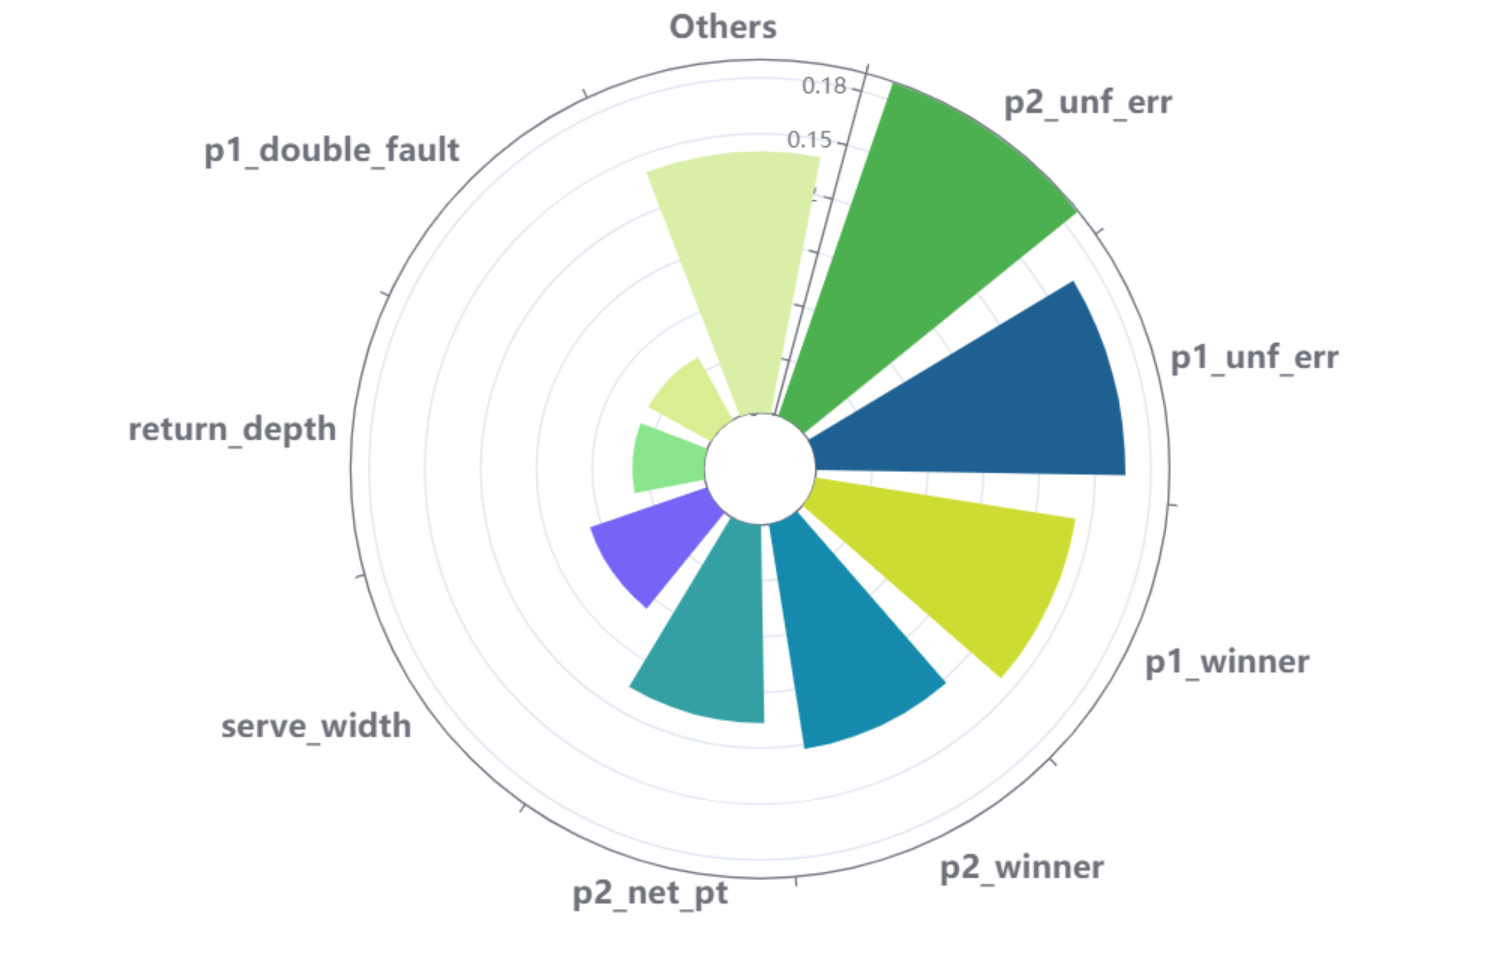
\includegraphics[width=0.8\textwidth]{figure/bar-polar-label-radial.png}
    % \vspace{-0.3cm}
    \caption{ Factors\textquotesingle~Contribution Based on Gradient Importance Analysis
    \textnormal{}}
    \label{fig:gradients_pie}
    % \vspace{-0.5cm}
\end{figure}

\subsection{Match recommendations based on momentum changes}

Here, we first analyze the quantification of momentum. Regarding the relative strength factors in this model, they are known quantities that allow us to assess the player's strength by comparing their historical performances with other players. Simultaneously, we can extract data from the opponent's match records, such as the timing and proportion of serving faults as the first server, as well as the increase in the number of points won over time. This information helps us understand when the player is more active and demonstrates stronger abilities during the match.

The MM-LSTM model provides the swing in the probability of winning from the beginning to the end, offering insights into the player's changing momentum. Here, the factors unrelated to the match time are analogized as "m", while those related to the match time are analogized as "v". The momentum "p" is influenced by changes in "m" of the same units, causing changes in "v" and directly affecting changes in "p". Therefore, both factors need to be considered in assessing the player's performance.

\begin{figure}[htbp]
    \centering
    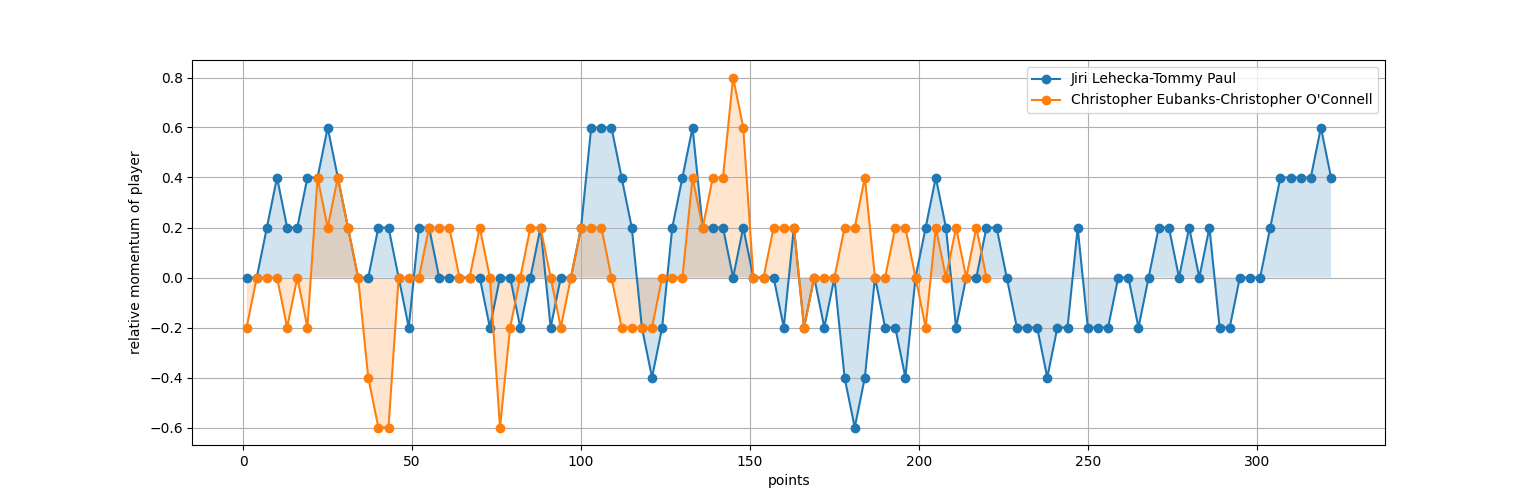
\includegraphics[width=1.1\textwidth]{figure/p_3_2_1.png}
    % \vspace{-0.3cm}
    \caption{The Momentum Indicator Changes in Two Matches
    \textnormal{}}
    % \label{fig:gradients_pie}
    % \vspace{-0.5cm}
\end{figure}



The figure above displays the relative momentum changes between the two players in two separate matches, with 0 as the starting point. It is evident that the trend of relative momentum changes is unpredictable. For instance, in the match represented by the blue line, Jini initially had the advantage but later allowed the opponent to come from behind. This swing is also reflected in the scoring situation.

Based on the correlation analysis between momentum and other factors, the following recommendations can be derived:



Psychological Considerations:
\begin{itemize}[label=\textbf{\normalsize$\bullet$}]
    \item As the saying goes, "make the best effort in the first push, weaken in the second, and exhaust in the third", it can be fair to conclude that, except for the first set, serving has no impact on winning that set.\cite{p321} For the first set, serving opportunities should be seized, and caution should be exercised when facing the opponent's serve. Do not become overconfident or careless due to an early advantage, as it may lead to failure in subsequent matches.
    \item Maintaining composure is crucial when facing uncontrollable outcomes with decisive consequences. The player's mentality directly determines the strength of their current momentum in the game. Unstoppable winning serves and unforced errors can be decisive, with a \(100\%\) impact on the outcome of the current exchange. Players should maintain a stable mindset, as the probability of such serves is very small, around \(5\%\), and subject to uncertainty over time. Therefore, there's no need to overly focus on such situations; learn to keep your composure. Additionally, after an unstoppable serve, the calculated probability of winning in the next five games increases to \(60\%\), highlighting the significant role of decisive factors in determining momentum.
    \item Stay humble and composed. In the data, when the current score is in favor of the player, the average probability of winning the point is \(26.81\%\), indicating that a lead may likely lead to failure. Be cautious in facing break points; winners facing break points tend to score more points, while losers struggle to maintain their level. Breaking and then holding serve is often more challenging than sailing smoothly with the wind.\cite{p322}
\end{itemize}

\begin{figure}[htbp]
    \centering
    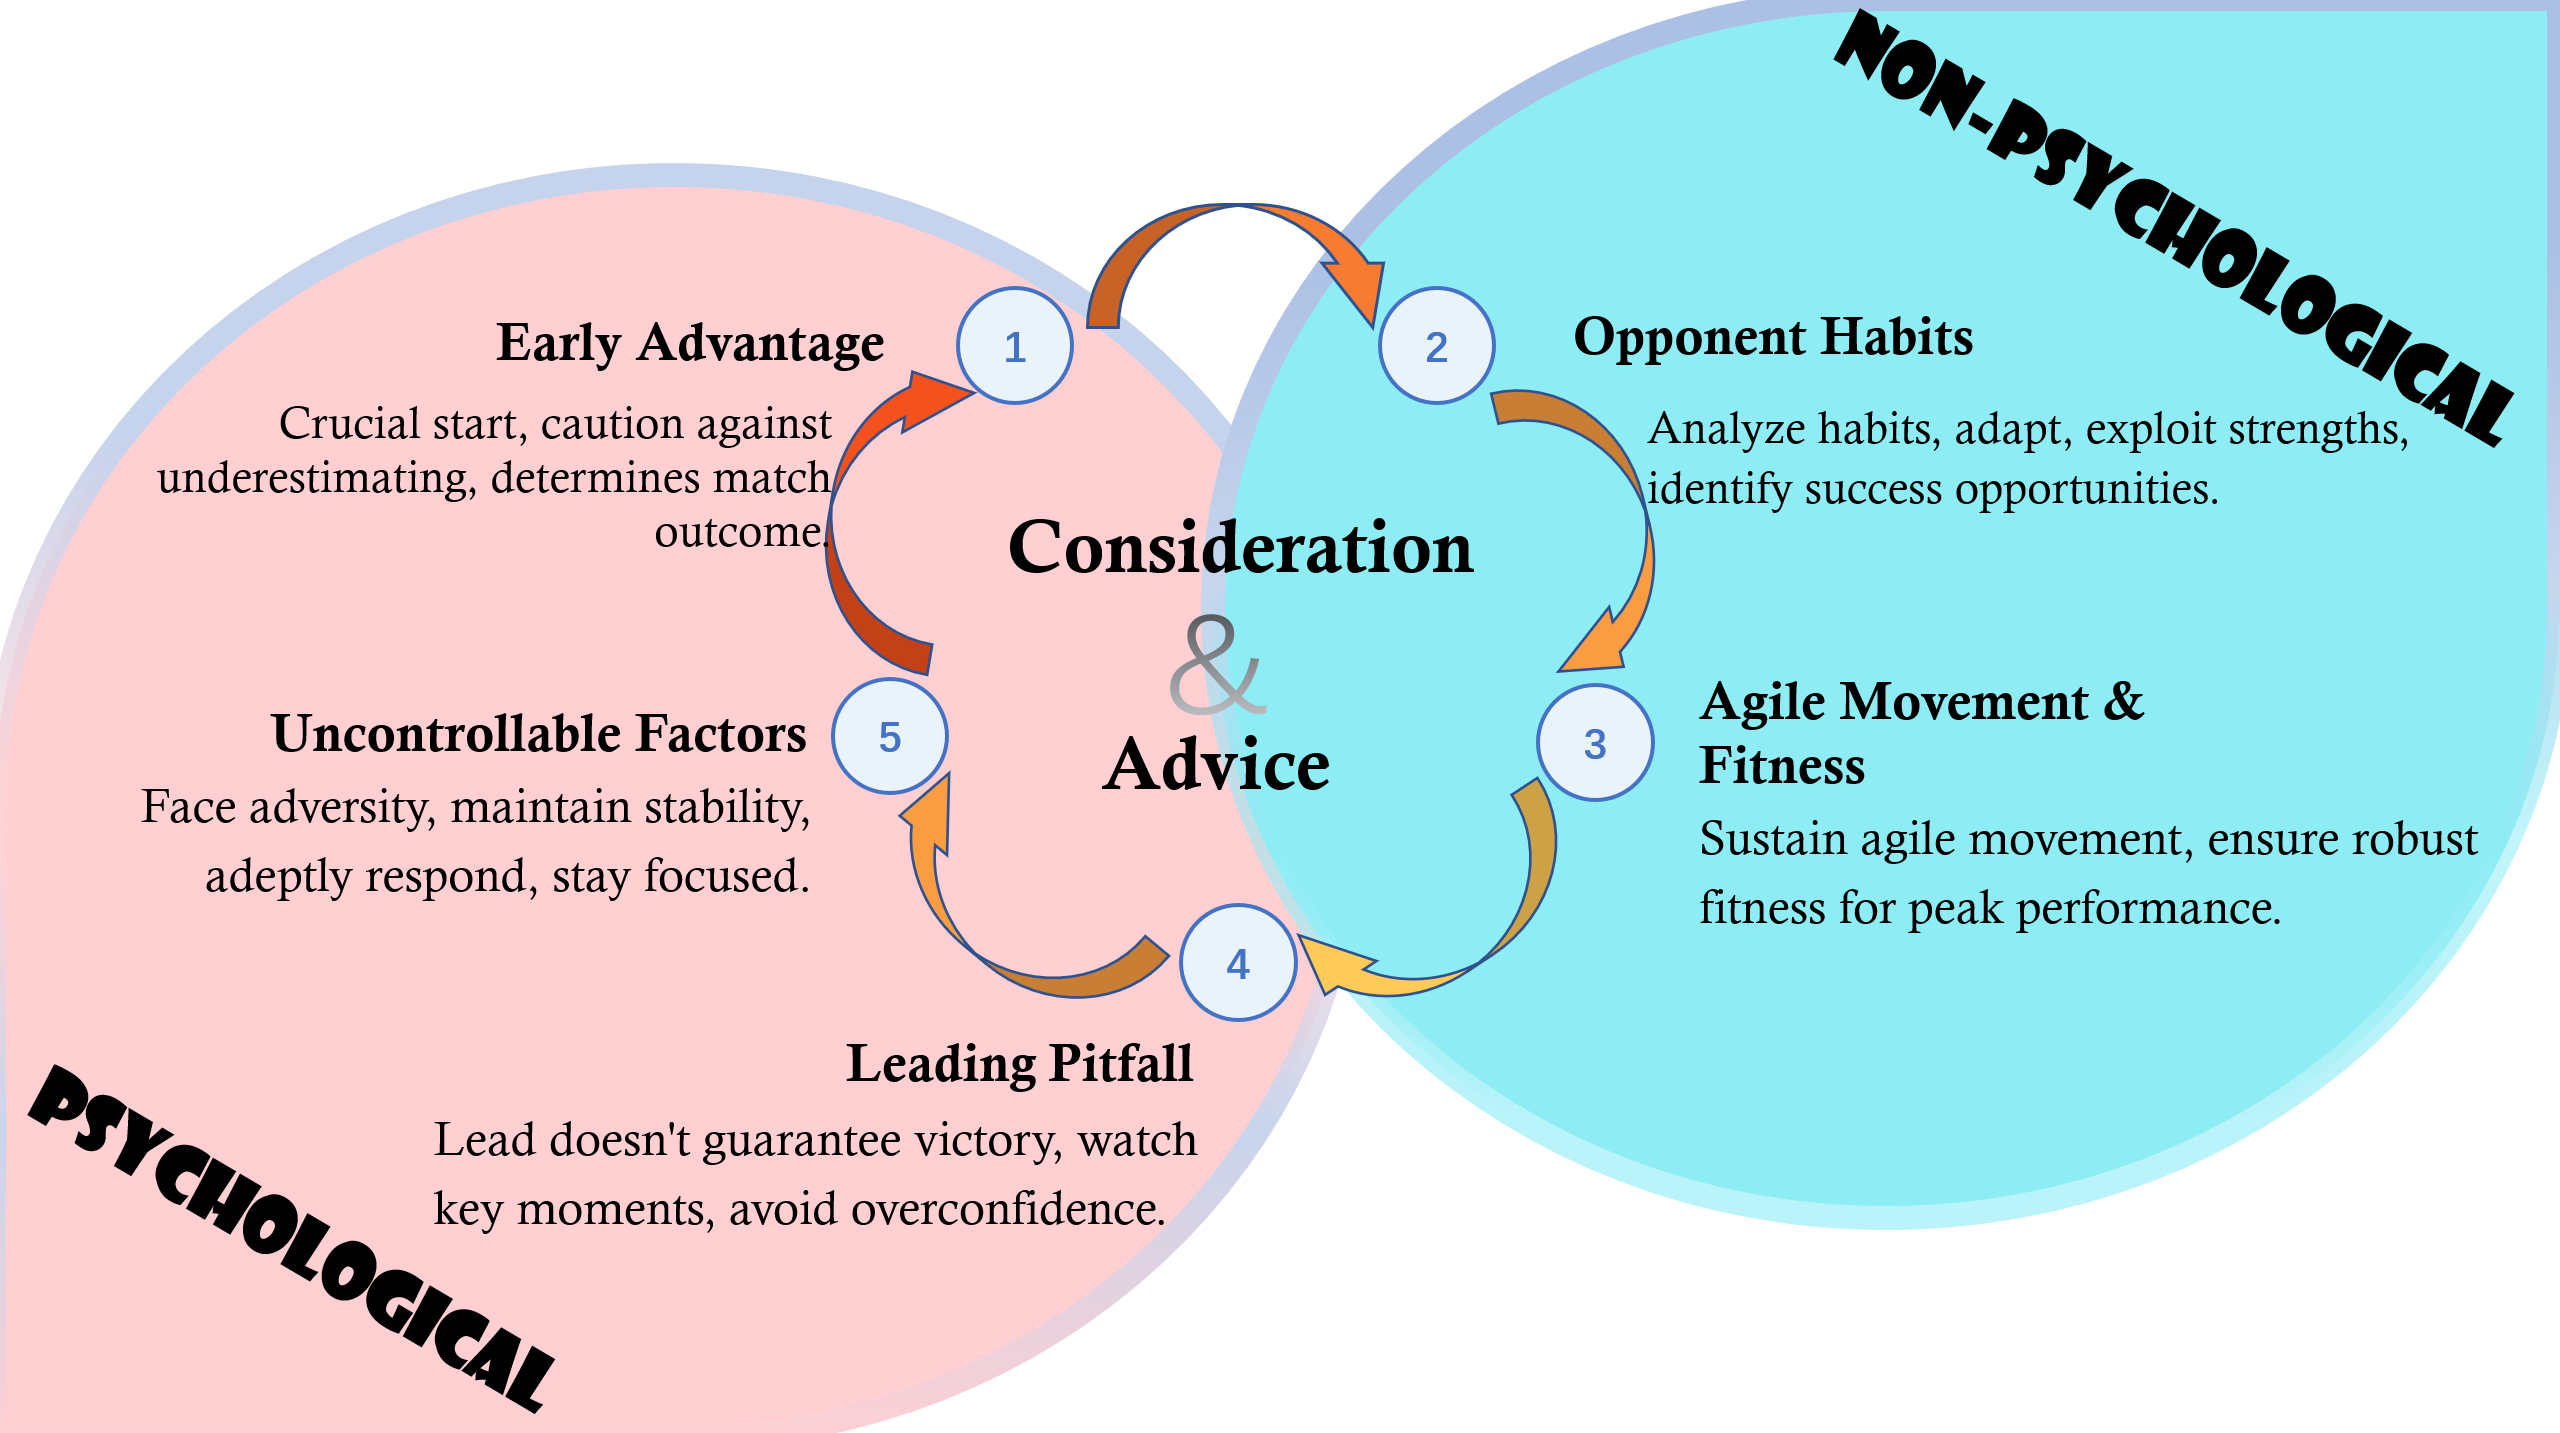
\includegraphics[width=0.95\textwidth]{figure/memo.png}
    % \vspace{-0.3cm}
    \caption{Suggestions for Athletes
    \textnormal{}}
    % \label{fig:gradients_pie}
    % \vspace{-0.5cm}
\end{figure}

Non-psychological Considerations:
\begin{itemize}[label=\textbf{\normalsize$\bullet$}]

\item Maintain flexibility on the court and avoid being confined to a specific area. According to data analysis, if a player is positioned at the net, their probability of scoring is \(69.88\%\), indicating a significant advantage in playing at the net. Additionally, when calculating the win rate with a running distance exceeding the average, it is \(48.75\%\), slightly lower than the average. This could be attributed to the physical exhaustion caused by increased running distance. However, in the statistics, it was found that the running distance in victorious matches tends to be slightly above the average. This suggests that while physical exhaustion has a minimal impact on victory, agile positioning and an active physique play a crucial role.

\item Carefully study the opponent's past match videos and data, paying attention to their strengths and weaknesses. Understand the opponent's playing style to formulate better tactics, including their preference for forehand or backhand, hitting power, speed, running distance, etc. According to the data, most players tend to prefer serving in the "w" direction, particularly favoring "CTL" near the sidelines, and their return shots usually have considerable depth. However, this is a general statistical observation for all players, and individual analysis should be conducted for specific opponents based on their historical data.
\end{itemize}

In conclusion, we believe that the most crucial aspect is to learn to control your own momentum. The main reason for the swings in momentum fundamentally depends on the changes in a player's strength over time on the court. By mastering and controlling these changes, you can achieve autonomy and make your momentum appear random while being controlled by yourself. This allows for the use of deceptive tactics to mislead opponents or to make continuous and aggressive progress, aiming for a decisive victory.






\section{Problem4: Validation and Expansion of MM-LSTM }

%%%%%%%%%%%%%%%
%% TODO
%%%%%%%%%%%%%%%
\subsection{Prediction of Momentum Swings}

Based on the MM-LSTM model established earlier, we used a match as the test set and obtained the corresponding output results:

\begin{figure}[htbp]
    \centering
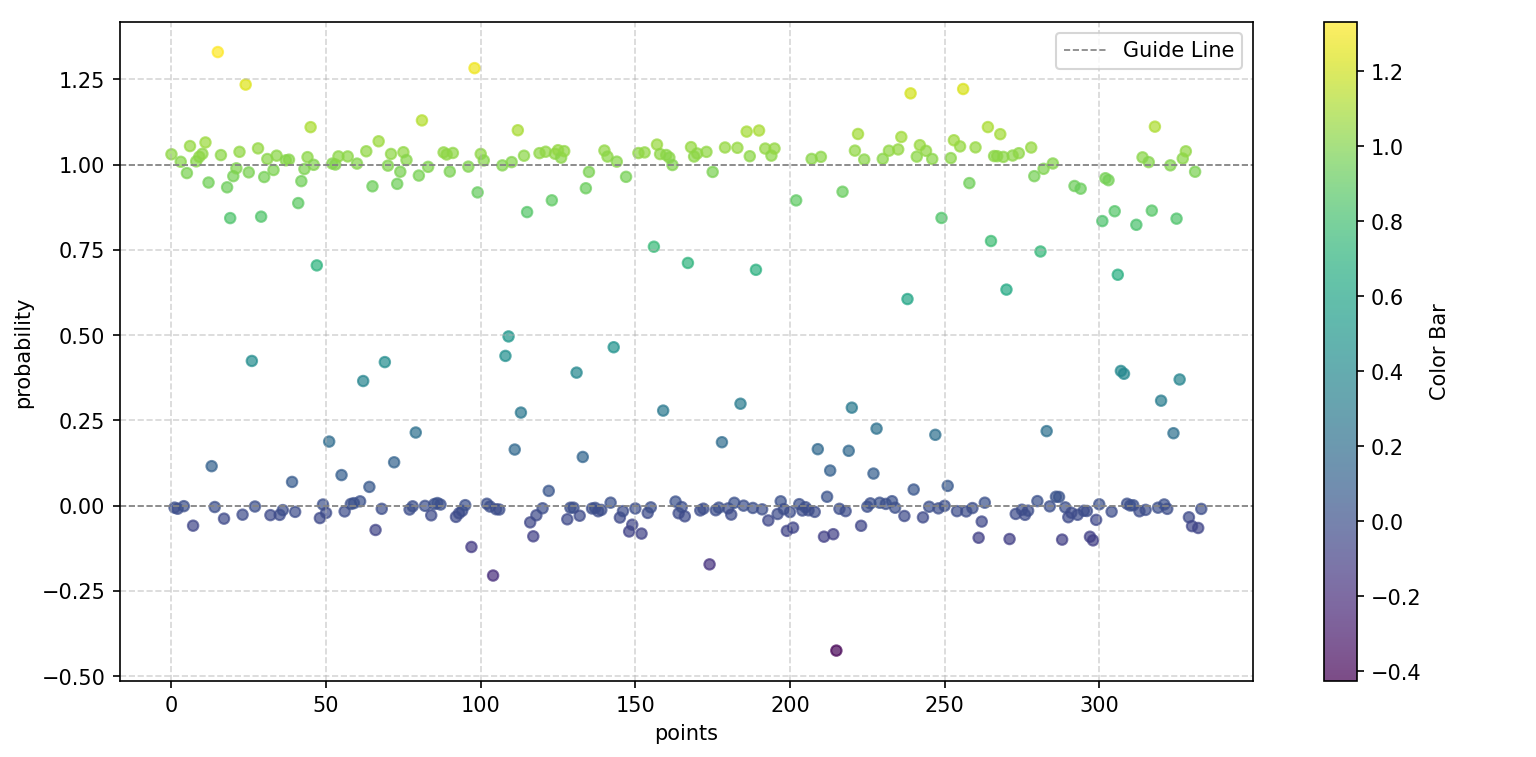
\includegraphics[width=1\textwidth]{figure/prediction_value_distribution.png}
    % \vspace{-0.3cm}
    \caption{Scatter Plot of Probability Values Predicted Using MM-LSTM Model}
    % \label{fig:gradients_pie}
    % \vspace{-0.5cm}
\end{figure}

We will calculate the probability value using the Equation \ref{eq:formula26}  and Equation \ref{eq:formula27} obtained from 5.1 to obtain $\eta_{\text{accuracy}} = 90.71\%$, the fitting effect is good. We will use Equation \ref{eq:formula25} to calculate the predicted relative slope curve of the fitted data, and plot the curve with the real data in the following figure:



\begin{figure}[htbp]
    \centering
     \hspace*{-1.2cm} % 负值表示左移
    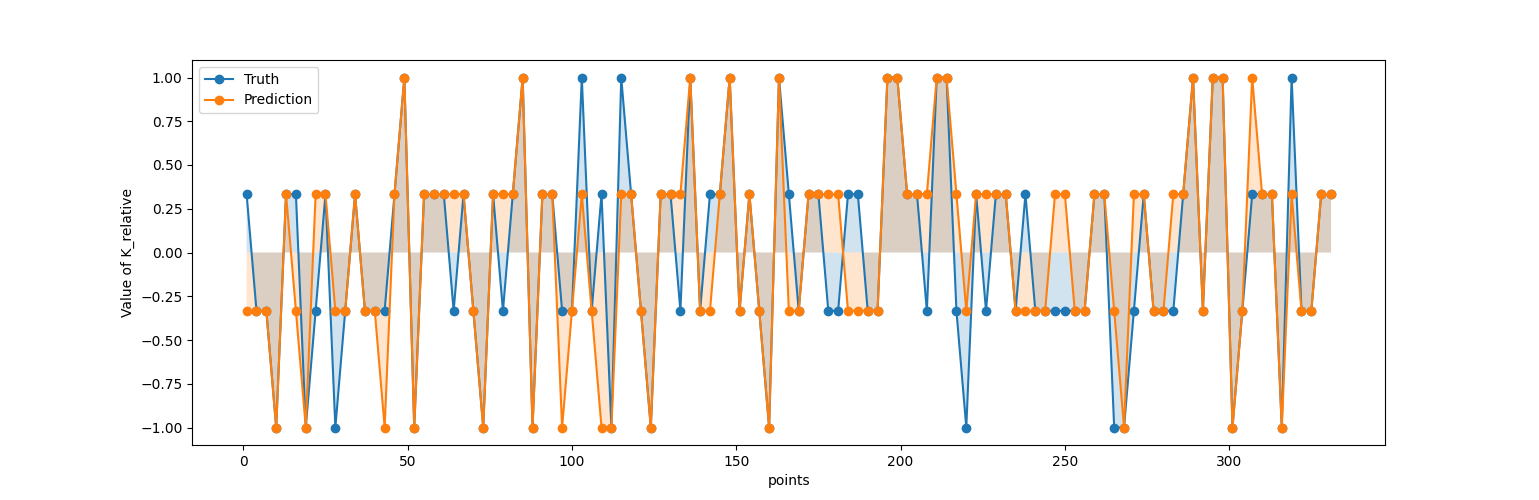
\includegraphics[width=1.1\textwidth]{figure/Figure_1.png}
    % \vspace{-0.3cm}
    \caption{The Fitting Effect of Momentum True Value and Predicted Value}
    % \label{fig:gradients_pie}
    % \vspace{-0.5cm}
\end{figure}

% 在以上图中我们可以得出,预测的动量波动曲线大部分均与真实动量波动曲线重叠,经测算拟合的决定系数R^{2}=61.51%,相关性与预测准确率相差较大可能是由于拟合系数与预测值是斜率和函数值的关系以及选取的时间段并不是一小部分而是一段时间导致的,在计算中当时间段points个数为3的时候拟合效果最好,我们认为过短导致图像波动过大拟合效果差,过长导致起伏都被均值化,无法体现出来。

In the above figures, we can observe that the predicted momentum fluctuation curve largely overlaps with the actual momentum fluctuation curve. The calculated coefficient of determination \(R^2\) is \(61.51\%\), indicating a moderate level of fit. The discrepancy between correlation and prediction accuracy could be attributed to the relationship between the fitting coefficient and predicted values, which involves the slope and function values. Additionally, the chosen time period is not a small subset but rather a segment, contributing to the observed difference. In the calculations, the best fitting performance is achieved when the number of data points in the time period is 3. We believe that too short a time span leads to excessive fluctuation in the graph, resulting in poor fitting performance. On the other hand, an overly long time span tends to average out the swings, making it challenging to capture the nuances.



\subsection{Future Model Influence Factors Analysis}
Based on the analysis of the above model prediction results, although it has reached 90.71\% belonging to the acceptable range of the predictive model; however, the model influence factor mainly focuses on the athletes' performance in the competition and its quantitative indexes, and it does not take into account many factors other than non-athletic performance factors. Therefore the assessment and quantification of subjective and objective factors of non-athletic performance is a direction that can be further optimized in the future model.

\subsubsection{Objective Factors}
The above model mainly analyzes the data of Wimbledon, where "serve is king", so the proportion of serve-related factors in the prediction model is high. However, in addition to Wimbledon, there are also the Australian Open, the US Open and the French Open among the four major tennis tournaments. Each tournament has its own unique characteristics, especially the venue factor is particularly prominent, such as Table \ref{tab:tennis_courts} is the analysis of the characteristics of different venues.

\begin{table}[htbp]
    \centering
    \caption{Tennis Court Characteristics and Associated Tournaments} 
    \vspace{8pt}
    \label{tab:tennis_courts}
    \begin{tabular}{c|cccc}
        \toprule[1.5pt]
        Court Type & Ball Speed & Return Height & Return Speed & Delegate Competition\\
        \midrule[1pt]
        Clay Courts & 1 & Very High & Medium & French Open \\
        Hard Courts & 2 & Stable & Fast & Australian Open \& U.S. Open \\
        Grass Courts & 4 & High & Very Fast & Wimbledon Championships \\
        Carpet Courts & 3 & Medium & Medium & ATP Indoor Race \\
        \bottomrule[1.5pt]
    \end{tabular}
\end{table}


Non-standardized court surface criteria are detrimental to the generality of the prediction model; the strong correlation between serve and rally speeds on grass at Wimbledon led players to generally adopt aggressive attacking strategies and serve to win; conversely, French Open players were more conservative, resulting in the longest average court time of the French Open matches. To enhance the predictive model, the training set can be extended to various court conditions. Ultimately, including court conditions as an influencing factor will improve the overall predictive accuracy of future models.

\subsubsection{Subjective Factors}
The subjective factors of the game are difficult to quantify, in which the psychological quality and the strength of the comparison is mutual influence, affecting the trend of the game. The level of the opponent indirectly affects the psychological state of the player, when encountering stronger opponents, may be nervous, resulting in malfunctioning; or there will be a "strong is strong" phenomenon can be over-performed. Correspondingly, when encountering weaker opponents, different psychological fluctuations will also occur, but the degree to which the psychological fluctuations affect the performance of different players varies. Therefore, it is very important for players to develop their self-regulation ability, anti-stress ability, and the ability to adapt to the venue from the experience of the tournament.

\subsection{Testing the generalizability of the model on table tennis matches}
To test the generalizability of our model across other sports, we collected data from the WTT 2024 table tennis matches. We trained and tested the model on a dataset consisting of 1515 table tennis matches. We partitioned 80\% of the data for training and reserved the remaining 20\% for testing. After training for 1000 epochs, our model achieved a prediction accuracy of 75.574\% on the test set, which did not reach the prediction accuracy achieved in tennis.


To analyze the reasons for the unsatisfactory performance of the model, we compared the collected data from the WTT 2024 matches with the data provided by MCM on the Wimbledon 2023 Gentlemen’s singles matches after the second round. We believe that the suboptimal prediction results in table tennis matches are due to the following two factors:

\begin{enumerate}
    \item The quantity of data collected for table tennis matches is relatively small. The tennis dataset comprises 7,285 data entries, whereas the table tennis dataset contains only 1,515 data entries, amounting to just 20.8\% of the tennis data in terms of entry count.
    \item The table tennis dataset lacks a variety of metrics compared to the tennis dataset. The table tennis data includes only the match ID, player names, and the scores of each player, without various in-game state metrics (such as "p1\_double\_fault" and "p2\_double\_fault"). Consequently, the total count of metrics in the table tennis data sums up to 6,060. In contrast, the tennis data, when counted by the number of metrics, totals 335,110. In summary, the sum of the table tennis metrics accounts for only 1.8\% of the total count of metrics in the tennis dataset.

\end{enumerate}

In conclusion, we believe that the MM-LSTM model we designed exhibits a certain degree of generality. However, its performance is constrained by the limited quantity of data. If more match data can be collected to allow the model to learn a greater variety of match-related information, there is substantial potential for improvement in model performance.

\section{Model Analysis}
\subsection{Strengths and Weaknesses}

\textit{\textbf{Strengths.}}
% \subsection{Strengths}
\begin{enumerate}
    \item \textbf{Close to real-world scenarios: }In problem 1, we utilized the three gate mechanisms and Cell state of LSTM to simulate the human processes of memory formation and forgetting, closely approximating real-life scenarios.

    \item \textbf{Temporal memory capability: }The LSTM model captures and remembers long-term dependencies through its Cell state, enabling it to effectively process long sequences of data and form a memory of the data throughout the competition process.
    \item \textbf{Momentum-based model representation: }In problem 2, we modeled the LSTM as a mathematical model based on momentum, providing a more formal analysis of the intrinsic relationship between the LSTM model and the momentum model.

    \item \textbf{Strong generalization capability: }We performed dimensionality reduction on the data from the competition, extracting some mutually independent factors to be used as inputs for the model, thereby enhancing its generalization capabilities when faced with new data.
    \item \textbf{Objective results: }The results of the model are quantifiable and can be described by mathematical representations so that speculative thinking is not required.
\end{enumerate}

% \subsection{Weaknesses}
\textit{\textbf{Weaknesses.}}
\begin{enumerate}
    \item \textbf{The momentum modeling is not comprehensive: }Due to the influence of many non-intuitive factors in the competition process, even though our LSTM model considers many factors in the game, it still cannot accurately model the momentum of players throughout the competition.
    \item \textbf{Insufficient prediction accuracy: }To further improve accuracy, we need to use more game data to enable our deep learning model LSTM to learn more information about the games.

\end{enumerate}


\subsection{Sensitivity Analysis}
To validate the model’s sensitivity, we simulated scenarios of missing data by selectively removing portions of the input data. Specifically, we sequentially excluded several variables that were identified to have the largest gradient contributions in Section \ref{sec:factor_contribution}. The model’s accuracy decreased by only 2\% when the variable with the greatest gradient contribution was removed. When five variables were excluded, the model still maintained an accuracy of 84\%. These results indicate that our model can adapt to partial data missingness, demonstrating strong robustness and resilience. The related experimental analysis results are presented in Figure \ref{fig:sensitivity_analysis}.

%%%%%%%%%
%%% 小标文字
%%%%%%%%%

\begin{figure}[htbp]
  \centering
  \subfigure[The accuracy of LSTM changing with the number of factors]
  {%
    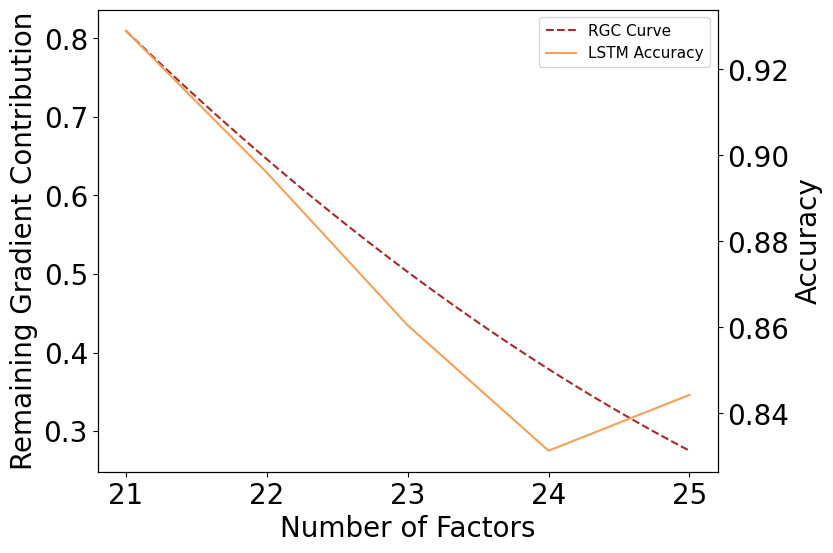
\includegraphics[width=0.45\textwidth]{figure/output2.png}
    \label{fig:lstm_acc_sensitivity_analysis}
  }
  % \hfill
  \hspace{1cm}
  \subfigure[The loss of LSTM changing with the number of factors]{%
    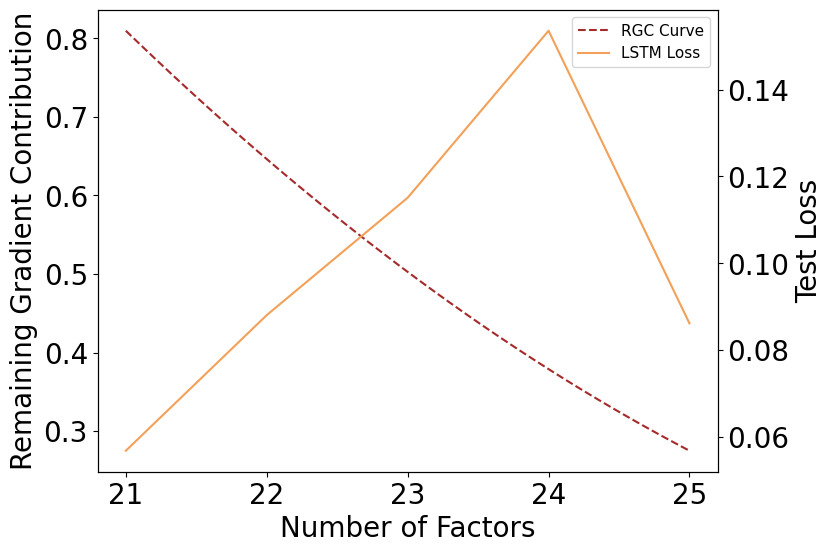
\includegraphics[width=0.45\textwidth]{figure/output1.png}
    \label{fig:lstm_loss_sensitivity_analysis}
  }
  \caption{Figures for Sensitivity Analysis}
  \label{fig:sensitivity_analysis}
\end{figure}
% \section{Model}
\lipsum[1-4] \cite{1}

\subsection{Equations}

%数学公式:
This is an equation:$$\frac{x}{y}=\frac{\sqrt[3]{x}}{\ln a}$$

This is an equation with number:(Heat Equation)\ref{e1}
\begin{equation}\label{e1}
	c\rho\frac{\partial u}{\partial t}=k\nabla^2u+f
\end{equation}

Matrix:
$$
\left( \begin{matrix}
1&		2&		3&		4\\
a&		b&		c&		d\\
x&		y&		z&		w\\
\alpha&		\beta&		\gamma&		\varphi\\
\end{matrix} \right) 
$$

Integral:

$$
\oint_l{pdx+qdy+rdz}
$$

Some Equation:
\begin{align*}
\cosh x = \frac {1}{2} (e^x + e^{-x}) &= \sum_{n = 0}^{\infty} \frac {x^{2n}}{(2n)!} \\
\sinh x = \frac {1}{2} (e^x - e^{-x}) &= \sum_{n = 0}^{\infty} \frac {x^{2n + 1}}{(2n + 1)!} \\
e^x &= \sum_{n = 0}^{\infty} \frac {x^n}{n!} = \lim_{n\to\infty} \left (1+\frac{x}{n} \right )^n\\
\end{align*}

\subsection{Figures}
This is a figure\ref{fig:comap-logo}:
\begin{figure}[h]
	\centering
	\includegraphics[width=0.7\linewidth]{"figure/comap logo"}
	\caption{Comap logo}
	\label{fig:comap-logo}
\end{figure}
\subsection{Equations}


% 描述运动员的动量p与时间之间的变化关系
\begin{equation}
p_i=\sum h_i(t)
\end{equation}
% 描述运动员具有的动量与各种因素之间的相互作用
\begin{equation}
\begin{aligned}
p_* & =\sum m_i v_i \\
& =\sum p_i
\end{aligned}
\end{equation}
% 描述先决条件中基础概率与发球手位置增加的概率
\begin{equation}
P_{\text {base }}=\frac{1}{2} \end{equation}\begin{equation}
R_{server}=0.173119165
\end{equation}
% 在这里指出发球位置对于胜利的影响
\[ Pserver = \left\{
\begin{array}{ll}
2 \cdot R_{server}, & \text{set\_no} = 1 \\
R_{server}, & \text{set\_no} = 2 \\
0, & \text{set\_no} > 2
\end{array}
\right.
\]

% 动量的基本定义式,其中m与运动员的实力等因素有关,不受比赛时间的进展而导致变化影响,v跟运动员在比赛时随时间进展而变化的因素有关
\begin{equation}
p=m v
\end{equation}
% 描述运动员获胜的概率表达式的基本构成,其中后者使用tanh激活函数将动量单位转化为概率单位,p1-p2表示两个运动员之间的动量差异,第二个为展开式,表示为影响动量的各种因素的差值,所以说影响胜利概率的是运动员之间的能力和各种其他因素的相对值
\begin{equation}
\begin{aligned}
& P_n=P_{\text {base }}+\frac{1}{2} \tanh \left(w \cdot\left({p_1-p_2}\right)\right) \\
& P_n=P_{\text {base }}+\frac{1}{2} \tanh \left(w \cdot\sum_{i=1}^n\left(p_{i 1}-p_{i 2}\right)\right).
\end{aligned}
\end{equation}
% 描述了运动员的动量变化原因,受各种因素的“趋势力”
\begin{equation}
p=\int_{t_1}^{t_2} F(t) d t
\end{equation}
% 以一个point为时间点,在这之间发生的v的变化原因是影响v的各种因素随时间的导数即变化趋势影响的
\begin{equation}v_{n}=v_{n-1}+\frac{\partial v}{\partial t} t
\end{equation}
% a就是加速度,他受具体因素影响,时间t,Q为之前赢得point的历史影响,s为体力消耗等其他因素
\begin{equation}a_{n}=g(t,Q,s)\end{equation}
% 描述了传统模型在描述概率上与LSTM模型预测值的等价性
\begin{equation}P_{n}=P_{base}+P_{server}\\+\alpha (p)=P_{LSTM}\end{equation}
% 描述了这部分概率的取值范围
\begin{equation}\frac{1}{2}\leq\alpha(p)+p_{server}\leq\frac{1}{2}\end{equation}
% 描述了第n次Q的取值
\begin{equation}Q_{n}=\begin{cases}1,win\\-1,fail\end{cases}\end{equation}
% 描述了相邻两次Q的递推关系
\begin{equation}History_{n}=History_{n-1}+\sum_{i=1}^{n-1}K_{i}Q_{i}\end{equation}
% 描述了第一次His的取值
\begin{equation}History_{1}=0\end{equation}
% ,Q与每一次Q之间的关系是一个函数History
\begin{equation}History_{n}=f\left(Q_{n-1},Q_{n-2},\ldots,Q_{1}\right)\end{equation}
% 这是输入门的变量取值
\begin{equation}I_{t}=\sigma(x_{t}\cdot k_{1}+h_{t-1}\cdot k_{2}+b_{1})\end{equation}
% 这是遗忘门的变量取值
\begin{equation}F_{t}=\sigma(x_{t}\cdot k_{3}+h_{t-1}\cdot k_{4}+b_{2})\end{equation}
% 这是输出门的变量取值
\begin{equation}O_{t}=\sigma(x_{t}\cdot k_{5}+h_{t-1}\cdot k_{6}+b_{3})\end{equation}
% 这是候选记忆状态的取值
\begin{equation}\tilde{C}_{t}=\tanh\left(x_{t}\cdot k_{7}+h_{t-1}\cdot k_{8}+b_{4}\right)\end{equation}
% 这是记忆状态的取值
\begin{equation}C_{t}=F_{t}\cdot C_{t-1}+I_{t}\cdot \tilde C_{t}\end{equation}
% 以下是带入整理的公式
\begin{equation}
\begin{gathered}
    H_{t} = O_{t} \cdot \tanh(C_{t}) = O_{t} \cdot \tanh\left(F_{t} \cdot C_{t-1} + I_{t} \cdot \tilde C_{t}\right) \\
    = \sigma(x_{t} \cdot k_{5} + h_{t-1} \cdot k_{6} + b_{3}) \cdot \tanh\left(\sigma(x_{t} \cdot k_{3} + h_{t-1} \cdot k_{4} + b_{2}) \cdot C_{t-1} \right.\\
    \quad \left. + \sigma(x_{t} \cdot k_{1} + h_{t-1} \cdot k_{2} + b_{1}) \cdot \tanh\left(x_{t} \cdot k_{7} + h_{t-1} \cdot k_{8} + b_{4}\right)\right)
\end{gathered}
\end{equation}
% 这是使用f代替后的表达式
\begin{equation}H_{t} = \sigma\left( f_{1}(x_{t}) \right) \cdot \tanh\left( \sigma(f_{2}(x_{t})) \cdot C_{t-1} + \sigma(f_{3}(x_{t})) \cdot \tanh(f_{4}(x_{t})) \right)\end{equation}
% 这是f的表达式
\begin{equation}
f_{i}(x_{t}) = x_{t}\cdot k_{a_{i}(t)} + h_{t-1} \cdot k_{b_{i}(t)} + b_{c_{i}(t)}
\end{equation}

% 在随机概率下,play1获胜的概率
\begin{equation}P_{1} = \frac{\left( P_{base} + P_{server} \right)\cdot m_{1}}{\left( P_{base} + P_{server} \right) \cdot  m_{1} +\left( P_{base} -P_{server} \right) \cdot m_{2} } 
\end{equation}
% 预测的准确率
\begin{equation}\eta_{accuracy}=\frac{N_{true}}{N_{toral}}=\frac{N_{true}}{N_{true}+N_{false}}\end{equation}


\newpage
\section{Memorandum}


\noindent To: The Global Professional Tennis Coach Association (GPTCA)

\noindent From: Team \#2416613 

\noindent Subject:  The Role of Momentum in Tennis Movement

\noindent Date: February 5, 2024 
\\

 \noindent Dear Officer of GPTCA:

From the model established by our team based on match data, we have found that Momentum plays a crucial role in tennis matches. Evaluating the Momentum indicator through model parameters in multiple matches for the same player allows for a high probability prediction of the score trend in subsequent matches. Furthermore, after neutralizing the skill gap between opposing players, the Momentum between different players in the same match shows a positive correlation with their performance.

Analyzing the predictive effects and understanding the changes in momentum, we have several important findings and suggestions that we hope will help improve the accuracy of your decisions.

\begin{enumerate}
\item Place special emphasis on the initial momentum shifts of both the opponent and one's own team during the match. Through the analysis presented earlier, it was observed that the momentum at the beginning of the game has a significant impact on the overall match. However, it is equally important to acknowledge the potential threat posed by momentum shifts resulting from underestimating the opponent.

\item In terms of model predictions, the undeniable improvement in accuracy of the MM-LSTM model compared to the fitted traditional models serves as compelling evidence for the powerful influence of momentum.

\item  For certain decisive factors, such as unstoppable winning serves or serving errors, their impact on momentum is significant and can influence players' attempts to build on success or stage a comeback during the match.
\end{enumerate}

Additionally, here are recommendations for players dealing with unexpected and decisive events in the flow of a tennis match:
\begin{enumerate}
\item  It's essential to break free from negative thinking early on and mentally fortify oneself like a warrior. Pay no mind to the opponent and strive to exhibit strength and resilience.

\item  Choosing the right moment to ignite one's inner passion undoubtedly proves more beneficial in the competition. Avoid expending energy too early and learn to manage time and energy wisely.

\item  During practice, keep score, so you can forget about the score during the match. In data analysis, it is evident that previous historical scores have a significant impact on the current situation. 
\end{enumerate}

In conclusion, in a match, robust physique, a stable and healthy mindset, appropriate strategic planning, and exceptional technical skills are all indispensable.

\begin{flushright}
    \textbf{Yours Sincerely,} \\
    \textbf{Team \#2416613}
\end{flushright}

\newpage
\begin{thebibliography}{99}
    \bibitem{insight}Briki W, Den Hartigh R J R, Markman K D, et al. How psychological momentum changes in athletes during a sport competition[J]. Psychology of Sport and Exercise, 2013, 14(3): 389-396.
    \bibitem{p_server}Klaassen F, Magnus J R. On the probability of winning a tennis match[J]. Medicine and Science in Tennis, 2003, 8(3): 10-11.
    \bibitem{p321} Magnus, Jan R., and Franc JGM Klaassen. "On the advantage of serving first in a tennis set: four years at Wimbledon." Journal of the Royal Statistical Society: Series D (The Statistician) 48.2 (1999): 247-256.
    \bibitem{p322}Meffert, Dominik, et al. "Tennis serve performances at break points: Approaching practice patterns for coaching." European journal of sport science 18.8 (2018): 1151-1157.
    % \bibitem{p421}An analysis of time factors in elite male tennis
    % players using the computerised scorebook for
    % tennis
\end{thebibliography}




\newpage
\section*{Appendices}
% \large{Appendices}
% \Large{Appendices}
% \LARGE{Appendices}

\textbf{\textit{\large{Core Code of LSTM}}}
\begin{lstlisting}
import torch
from torch import nn
class LSTMModel(nn.Module):
    def __init__(self, input_size, hidden_size, num_layers, output_size):
        super(LSTMModel, self).__init__()
        self.hidden_size = hidden_size
        self.num_layers = num_layers
        self.lstm = nn.LSTM(input_size, hidden_size, num_layers, batch_first=True)
        self.fc = nn.Linear(hidden_size, output_size)
    def forward(self, x):
        h0 = torch.zeros(self.num_layers, x.size(0), self.hidden_size).to(x.device)
        c0 = torch.zeros(self.num_layers, x.size(0), self.hidden_size).to(x.device)
        h0 = h0.squeeze(0)
        c0 = c0.squeeze(0)
        out, _ = self.lstm(x, (h0, c0))
        out = self.fc(out[:, -1, :])
        return out

\end{lstlisting}

% \begin{lstlisting}[language=Python]
% def hello_world():
%     print("Hello, world!")
% \end{lstlisting}

% \lipsum[1-2]
% \subsection{Appendices 2}
% \lipsum[1-2]
% \begin{ReportAiUse}{9}
% \bibitem{AI1}
% Bing AI\\
% Query1: write a sort algorithm\\
% Output: Sure, I can help you with that. Here is a simple implementation of the selection sort algorithm in Python:
% \begin{lstlisting}[language=python]
% def selection_sort(arr):
%     for i in range(len(arr)):
%         min_idx = i
%         for j in range(i + 1, len(arr)):
%             if arr[min_idx] > arr[j]:
%                 min_idx = j
%         arr[i], arr[min_idx] = arr[min_idx], arr[i]
%     return arr
% \end{lstlisting}
% This algorithm sorts an array by repeatedly finding the minimum element from the unsorted part of the array and putting it at the beginning. \href{https://www.geeksforgeeks.org/sorting-algorithms/}{The time complexity of this algorithm is O($n^2$)}.

% There are many other sorting algorithms available such as bubble sort, insertion sort, merge sort, quick sort, heap sort, and more. Each of these algorithms has its own advantages and disadvantages. You can learn more about them on GeeksforGeeks and Programiz.

% I hope this helps!

% \bibitem{AI2}
% OpenAl Enie (Nov 5, 2023 version, Ernie 4.0)\\
% Query1: <insert the exact wording of any subsequent input into the Al tool>\\
% Output: <insert the complete output from the second query>

% \bibitem{AI3}
% Github CoPilot (Feb 3, 2024 version)\\
% Query1: <insert the exact wording you input into the Al tool>\\
% Output: <insert the complete output fron the Al tool>

% \bibitem{AI4}
% Google Bard (Feb 2,2024 version)\\
% Query: <insert the exact wording of your query>\\
% Output: <irsert the complete output from the Al tool>

% \bibitem{AI5}
% Bing AI\\
% Query: write a FFT algorithm\\
% Output: Sure, here is a Python implementation of the Fast Fourier Transform (FFT) algorithm:
% \begin{lstlisting}[language=python]
% import numpy as np

% def fft(x):
%     n = len(x)
%     if n == 1:
%         return x
%     even = fft(x[0::2])
%     odd = fft(x[1::2])
%     T = [np.exp(-2j * np.pi * k / n) * odd[k] for k in range(n // 2)]
%     return [even[k] + T[k] for k in range(n // 2)] + [even[k] - T[k] for k in range(n // 2)]
% \end{lstlisting}
% The FFT is a widely used algorithm for computing the \textbf{Discrete Fourier Transform (DFT)} of a sequence. It reduces the number of computations needed from O(n$^2$) to O(n log n) 12. The basic idea of the FFT is to apply divide and conquer. We divide the coefficient vector of the polynomial into two vectors, recursively compute the DFT for each of them, and combine the results to compute the DFT of the complete polynomial 3.

% I hope this helps!

% \end{ReportAiUse}
% \end{appendices}
\newpage
% 在希望应用该样式的页面上调用
\thispagestyle{nopagenum}
\begin{center} % 开始居中环境
\textbf{ % 开始加粗
\underline{ % 开始添加下划线
\large{Report On use of AI}
}} % 结束下划线和加粗
\end{center} % 结束居中环境
% \section{Report On use of AI}
\begin{enumerate}
\item OpenAI ChatGPT (Feb 6, 2024 version,ChatGPT-3.5)

Query1: Could you please explain the exact interpolation method and formula?

Output: Certainly! Interpolation is a technique used to estimate values between two known values or data points. There are various interpolation methods, and the choice of method depends on the nature of the data and the desired level of accuracy. I'll explain two commonly used interpolation methods: linear interpolation and Lagrange interpolation.

1. \textbf{Linear Interpolation:}
   Linear interpolation is a simple method that assumes a linear relationship between two adjacent data points. Given two points \((x_1, y_1)\) and \((x_2, y_2)\), the linear interpolation formula for estimating the value \(y\) at a point \(x\) between \(x_1\) and \(x_2\) is:
   \[ y = y_1 + \frac{{(x - x_1) \cdot (y_2 - y_1)}}{{x_2 - x_1}} \]

2. \textbf{Lagrange Interpolation:}
   Lagrange interpolation uses a polynomial to fit the data points. For \(n+1\) data points \((x_0, y_0), (x_1, y_1), \ldots, (x_n, y_n)\), the Lagrange interpolation polynomial is given by:
   \[ P(x) = \sum_{i=0}^{n} y_i \cdot L_i(x) \]
   where \(L_i(x)\) is the Lagrange basis polynomial:
   \[ L_i(x) = \prod_{j=0, j \neq i}^{n} \frac{{x - x_j}}{{x_i - x_j}} \]

   The Lagrange polynomial passes through all the given data points and can be used to estimate the function values at points between the given data.

These formulas provide a simplified explanation of linear and Lagrange interpolation. In practice, for more complex data, other interpolation methods like spline interpolation or polynomial interpolation of higher degree might be used, depending on the specific requirements and characteristics of the dataset.


\item OpenAI ChatGPT (Feb 4, 2024 version,ChatGPT-3.5)

Query1: Gradient calculation formula

Output: In mathematics and computation, the gradient is typically a vector that represents the rate of change or slope of a function at a specific point. For a scalar function \(f(x)\), its gradient \(\nabla f(x)\) can be computed through partial derivatives. If \(f(x)\) is a multivariable function, the gradient is a vector where each component corresponds to the partial derivative with respect to the respective variable.

The general formula for gradient computation is as follows:

For a scalar function \(f(x_1, x_2, ..., x_n)\), its gradient \(\nabla f\) is a vector containing partial derivatives:

\[ \nabla f = \left( \frac{\partial f}{\partial x_1}, \frac{\partial f}{\partial x_2}, ..., \frac{\partial f}{\partial x_n} \right) \]

Here, each \(\frac{\partial f}{\partial x_i}\) represents the partial derivative with respect to the variable \(x_i\).

If you have a specific function \(f(x_1, x_2, ..., x_n)\), you can use this formula to compute its gradient.

\end{enumerate}

\thispagestyle{nopagenum}




%%%%%%%%%%%%%%%%%%%%%%%%%%%%%%


\end{document}
% \end

